\section{System Analysis and Design}
\subsection{System Architecture}

To visualize data flows and the separation of concerns across technology components in the Online Library Management System, the overall structure is modeled via the architecture diagram below:

\begin{figure}[H]
	\centering
	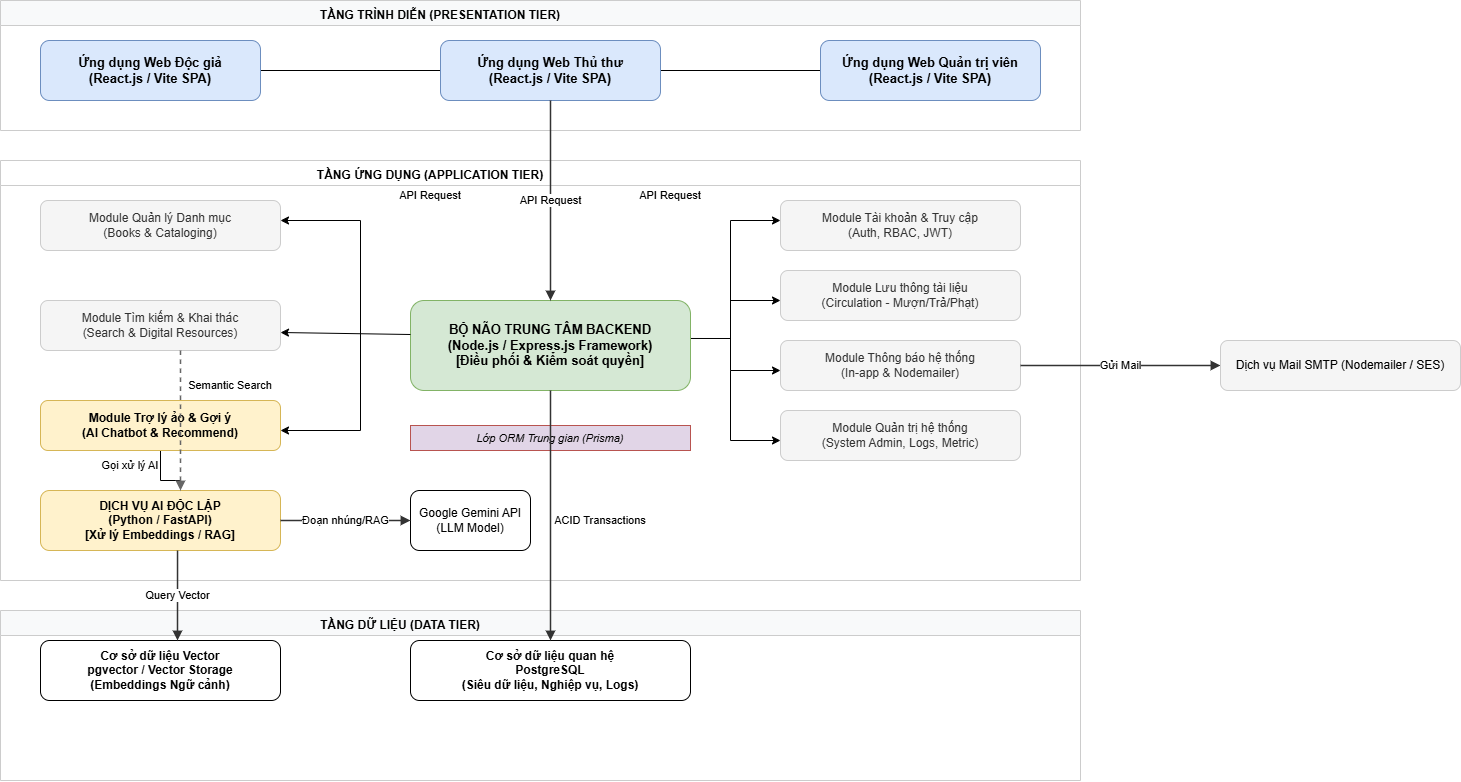
\includegraphics[width=0.6\linewidth]{Images/kientruchethong.png}
	\vspace{10pt}
	\caption{Overall System Architecture Diagram of the Online Library Management System}
	\label{fig:system_architecture}
\end{figure}

Overall, the architecture of the Online Library Management System is built upon a standard Three-Tier Architecture, combined flexibly with a Service-Oriented Architecture (SOA) paradigm to optimize independent Artificial Intelligence workloads. The three foundational tiers of the project comprise: the Presentation Tier, Application Tier, and Data Tier.

Applying this model ensures clear separation of responsibilities between user interface interactions, library business logic, and database management systems. Thanks to high inter-tier decoupling, our team can easily maintain or upgrade individual components independently (such as optimizing AI algorithms or updating the web interface) without disrupting core underlying operational processes.

\subsubsection{Presentation Tier}
Serving as the direct touchpoint for end-users, this tier is implemented as a robust Single Page Application (SPA) utilizing the React.js library and Vite build tool. The interface is tailored with strict Role-Based Access Control (RBAC) across three distinct user roles: Reader, Librarian, and Administrator (Admin).

All user interactions—including searching for documents, submitting checkout requests, chatting with the AI assistant, or executing librarian operations—are captured, asynchronously processed, and converted into standardized RESTful API requests before transmission to the central processing tier.

\subsubsection{Application Tier}
Functioning as the core orchestration hub, the Application Tier receives, processes, and executes complex business logic required for a smart library system. This tier operates primarily within a Node.js environment paired with the Express.js framework, while integrating a decoupled Python service (FastAPI) dedicated to high-performance AI workloads. To ensure modularity and scalability, the backend is partitioned into 7 functional modules matching system business domains:

\begin{itemize}
	\item \textbf{Account and Access Management Module:} Protects system security via Role-Based Access Control (RBAC) combined with password hashing. The system employs JSON Web Tokens (JWT) to securely manage user sessions. Additionally, this module manages personal user profiles, OTP verification codes, and activity audit logs for readers and library staff.

	\item \textbf{Book Catalog Management Module:} Organizes hierarchical category structures (\texttt{Category}) and stores book metadata (\texttt{Book}). This sub-system assists librarians in automated cataloging by integrating third-party APIs (Open Library, Google Books API) for ISBN metadata fetching.

	\item \textbf{Document Circulation Management Module:} Handles the full lifecycle of physical item checkouts and returns. It tracks stack availability per copy (\texttt{PhysicalCopy}) via barcodes, automates reservation queues (\texttt{Reservation}), calculates online renewal eligibility, enforces fine rules (\texttt{Fine}) for overdue returns, and orchestrates inter-branch item transfers.

	\item \textbf{Search and Resource Exploitation Module:} Provides advanced keyword and semantic search filtering to optimize query performance across the book catalog.

	\item \textbf{Virtual Assistant and Recommendation Module:} Operates as a decoupled high-performance microservice leveraging Large Language Models (LLMs) via Google Generative AI (Gemini) APIs. Capabilities include: Natural language Semantic Search, AI document summarization, preference prediction algorithms for personalized recommendations, and a 24/7 Virtual Assistant Chatbot.

	\item \textbf{Notification Module:} Automates real-time user communications. The system listens for system events (due date reminders, fine assessments, hold availability) to dispatch multi-channel notifications via in-app alerts and automated emails using Nodemailer.

	\item \textbf{System Administration Module:} Provides administrative tools for system management, including dynamic system configuration key-values (\texttt{system\_configs}), branch network management, real-time metric dashboards (\texttt{Dashboard Metrics}), automated database backups, and snapshot disaster recovery.
\end{itemize}

To maximize development velocity and type safety, the Application Tier utilizes \textbf{Prisma ORM} as the data access layer. Capitalizing on TypeScript's strict static type checking, Prisma catches query syntax errors during compile time. Prisma Migrate manages database schema versioning, ensuring seamless automated schema synchronization between development and production environments.

\subsubsection{Data Tier}
The data storage layer provides persistent, secure, and ACID-compliant storage for all system records. It comprises two specialized database stores:

\begin{itemize}
	\item \textbf{Relational Database (PostgreSQL):} For library operations requiring strict financial transaction accuracy and concurrent consistency (e.g., decrementing physical inventory while generating loan tickets), \textbf{PostgreSQL} is selected for its robust ACID compliance. High-performance index structures ensure low latency under heavy query loads. Additionally, all sensitive state-mutating actions write automated entries to audit logs (\texttt{AuditLog}).

	\item \textbf{Vector Database (pgvector):} To power Retrieval-Augmented Generation (RAG) and semantic search in AI modules, the data tier incorporates vector storage mechanisms. Text summaries, book metadata, and digital document chunks converted into high-dimensional vector embeddings are stored and queried using Cosine Similarity directly in `pgvector`.
\end{itemize}

\subsection{Database Design}
\subsubsection{Entity Descriptions}

\begin{table}[H]
	\centering
	\begin{tabular}{|p{4cm}|p{4cm}|p{7cm}|}
		\hline
		\textbf{Entity Category} & \textbf{Entity Name}   & \textbf{Description}                                                                   \\ \hline

		\multirow{5}{*}{User \& Access Control}
		                         & users                  & Stores user account profiles including readers, librarians, and system administrators. \\ \cline{2-3}
		                         & roles                  & Manages system roles and authorization permissions (Admin, Librarian, Reader).         \\ \cline{2-3}
		                         & otp\_tokens            & Stores OTP tokens for login authentication, password resets, and MFA.                  \\ \cline{2-3}
		                         & notification\_settings & Stores user notification preferences across Email, SMS, and In-app channels.           \\ \cline{2-3}
		                         & notifications          & Manages system notifications dispatched to users (due date alerts, hold notices).      \\ \hline

		\multirow{5}{*}{Library Resources}
		                         & books                  & Stores metadata records for books, journals, and digital academic materials.           \\ \cline{2-3}
		                         & categories             & Manages hierarchical category classifications for subjects and disciplines.            \\ \cline{2-3}
		                         & physical\_copies       & Tracks physical copy instances, circulation statuses, and shelf locations.             \\ \cline{2-3}
% 		                         & digital\_resources     & Stores digital assets (E-books, PDF files) for online streaming and reading.           \\ \cline{2-3}
% 		                         & digital\_access\_logs  & Logs user digital resource reading sessions for analytics and DRM auditing.            \\ \hline

		\multirow{5}{*}{Library Circulation}
		                         & borrow\_records        & Tracks loan and return lifecycles for physical library items.                          \\ \cline{2-3}
		                         & reservations           & Manages item hold reservation queues when copies are out of stock.                     \\ \cline{2-3}
		                         & fines                  & Manages overdue fines and penalty fee assessments.                                     \\ \cline{2-3}
		                         & branches               & Stores branch library profiles and campus location metadata.                           \\ \cline{2-3}
		                         & branch\_transfers      & Manages physical copy transfers between branch libraries.                              \\ \hline

		\multirow{2}{*}{Interaction \& Reviews}
		                         & reviews                & Stores user ratings, reviews, and feedback on library materials.                       \\ \cline{2-3}
		                         & chat\_history          & Stores conversation transcripts between users and the AI Chatbot assistant.            \\ \hline

		\multirow{2}{*}{System \& Administration}
		                         & audit\_logs            & Records administrative and security audit events for system compliance.                \\ \cline{2-3}
		                         & system\_configs        & Stores global dynamic configuration parameters for system operation.                   \\ \hline
	\end{tabular}
	\caption{System Entities and Database Definitions}
	\label{tab:entity-description}
\end{table}

\subsubsection{Enhanced Entity-Relationship Diagram (EERD)}

\begin{figure}[H]
	\centering
	\includegraphics[width=\linewidth]{Images/ERD.png}
	\vspace{10pt}
	\caption{EERD Diagram of the Online Library Management System}
	\label{fig:erd_account}
\end{figure}

Based on the Enhanced Entity-Relationship Diagram (EERD), the system operational workflows are partitioned across three primary user roles:

\paragraph{Reader Role}
End-users interacting with the platform to search, borrow, and read physical and digital items:
\begin{itemize}
	\item \textbf{Account Management \& Security:} Executes multi-factor authentication via OTP tokens (\texttt{otp\_tokens}); configures notification channels (Email, SMS, In-app) in \texttt{notification\_settings}.
	\item \textbf{Physical Borrowing \& Catalog Search:} Searches and browses categories (\texttt{categories}). Borrows physical materials with loan records tracked in \texttt{borrow\_records}.
	\item \textbf{Physical Borrowing \& Returns:} Submits loan requests and tracks borrowing lifecycles in \texttt{borrow\_records} tied to specific copies (\texttt{physical\_copies}).
	\item \textbf{Reservation Queue Management:} When items are out of stock, places hold reservations (\texttt{reservations}) with automated queue positioning via \texttt{queuePosition}.
	\item \textbf{Feedback \& Ratings:} Submits star ratings and reviews (\texttt{reviews}); chats with the AI Virtual Assistant (\texttt{chat\_history}); views and pays fine ledgers (\texttt{fines}).
\end{itemize}

\paragraph{Librarian Role}
Operational staff managing physical stacks, catalog entries, and counter circulation:
\begin{itemize}
	\item \textbf{Physical Stack Management:} Manages catalog records (\texttt{books}), copy availability (\texttt{status}), physical condition (\texttt{condition}), and shelf location (\texttt{location}) in \texttt{physical\_copies}.
	\item \textbf{Circulation Desk Processing:} Scans barcodes (\texttt{barcode}) and reader cards (\texttt{readerCode}), updating \texttt{borrow\_records}.
	\item \textbf{Reservation Queue Orchestration:} Monitors reservation queues (\texttt{reservations}), updating copy statuses upon return and alerting next patrons.
	\item \textbf{Inter-Branch Logistics:} Approves and tracks item transfer tickets between branch libraries via \texttt{branch\_transfers}.
	\item \textbf{Fine Assessment \& Waivers:} Reviews overdue penalties in \texttt{fines}, possessing authorization to grant fine waivers (\texttt{waivedById}, \texttt{waivedReason}).
\end{itemize}

\paragraph{Administrator Role}
System administrators holding global configuration, user security, and audit privileges:
\begin{itemize}
	\item \textbf{User Management \& RBAC:} Activates, locks, or suspends accounts (\texttt{users}), managing failed login limits (\texttt{failedLoginCount}) and role permissions (\texttt{roles}).
	\item \textbf{Infrastructure Administration:} Manages branch network configurations (\texttt{branches}) and assigns branch managers (\texttt{managerId}).
	\item \textbf{Global Parameters:} Configures operational system policies via \texttt{system\_configs} (daily fine rates, loan limits, max file upload sizes).
	\item \textbf{System Audit \& Compliance:} Monitors audit logs (\texttt{audit\_logs}) for data security and regulatory compliance.
\end{itemize}

\subsubsection{Database Schema}
\begin{figure}[H]
	\centering
	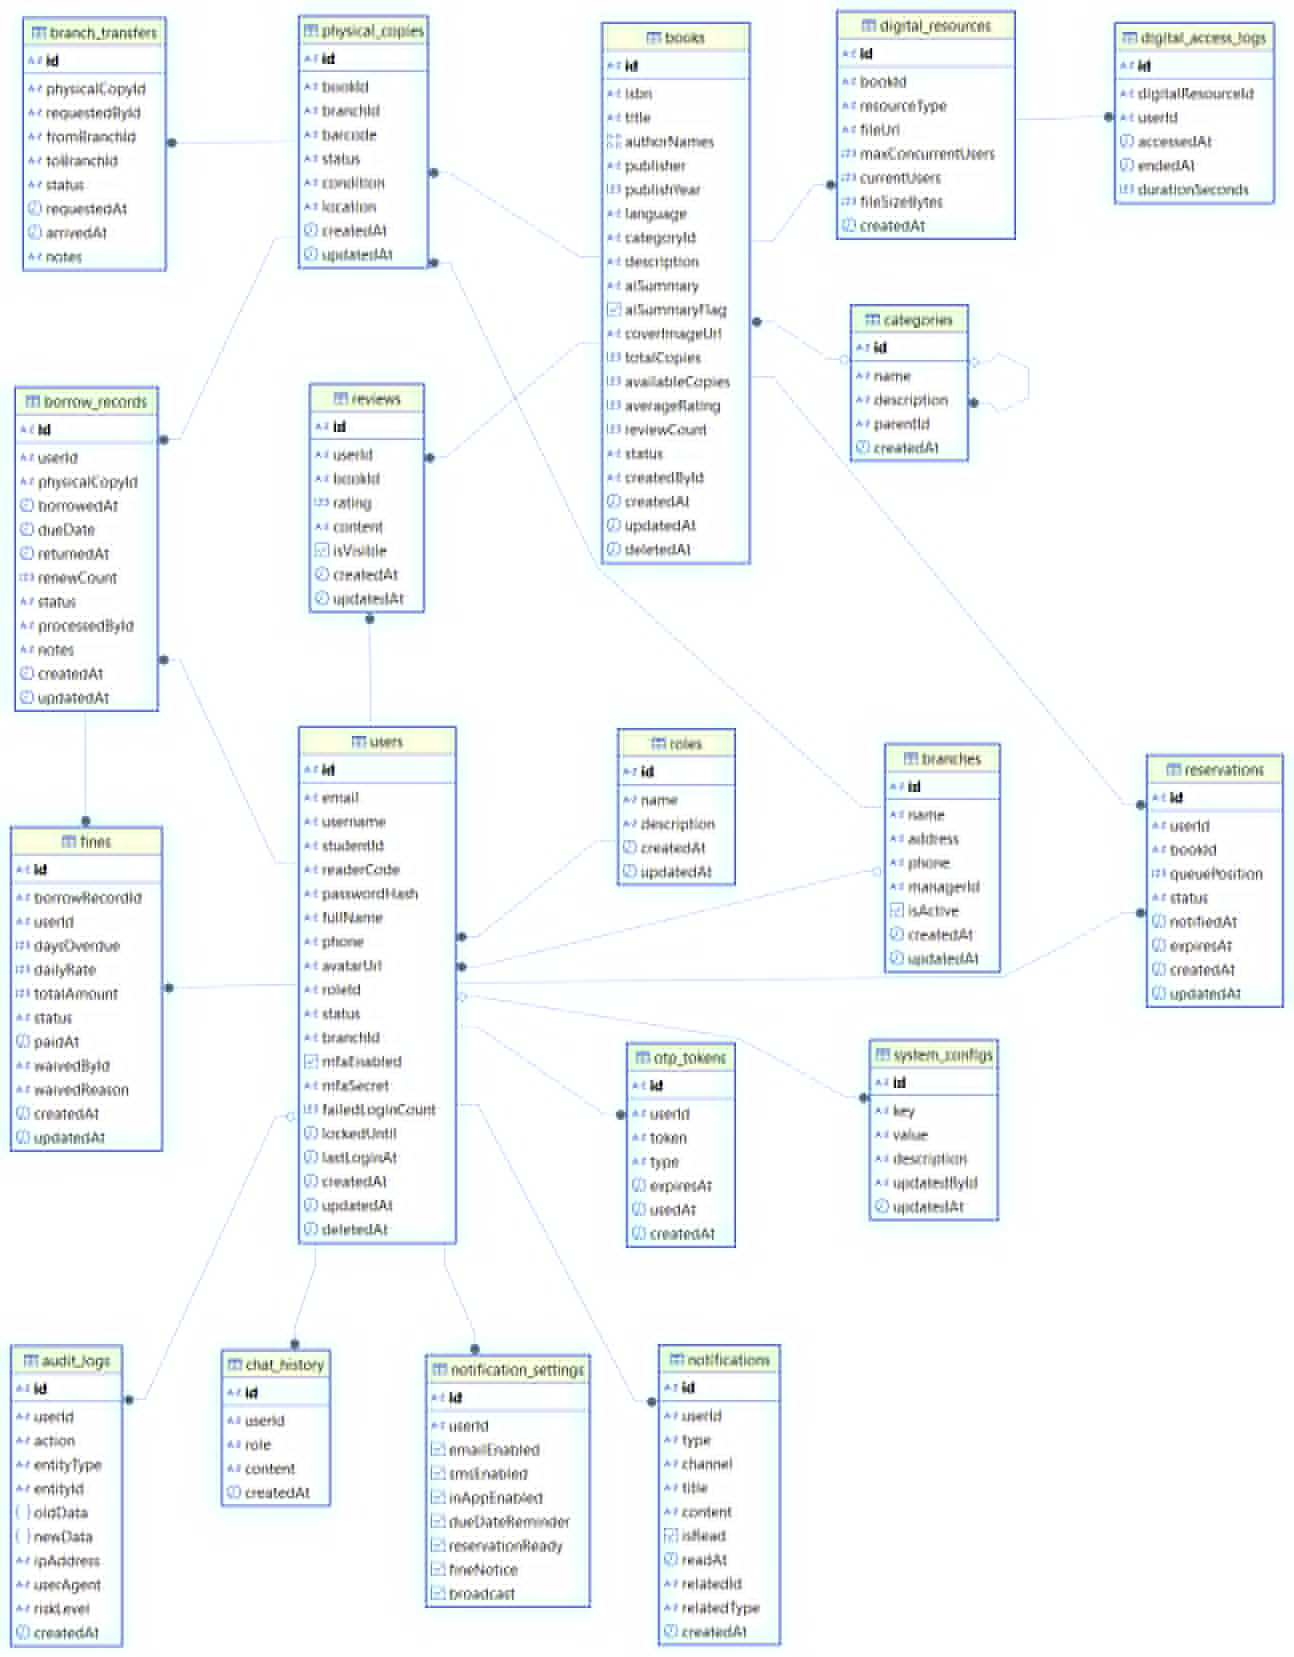
\includegraphics[width=0.6\linewidth]{Images/db.jpg}
	\vspace{10pt}
	\caption{Relational Database Schema for the Online Library Management System}
	\label{fig:database_account}
\end{figure}
The schema above represents the relational structure implemented on PostgreSQL.

User accounts are centralized in the \texttt{users} table, linked to \texttt{roles} via foreign key \texttt{roleId} for RBAC permission checks. Security flags such as \texttt{status}, \texttt{failedLoginCount}, and \texttt{lockedUntil} enforce login security constraints.

Remaining tables map directly to the entity definitions and EERD relationships detailed above.

\subsection{Class Diagram}

\subsubsection{Account and Access Management}

\begin{figure}[H]
	\centering
	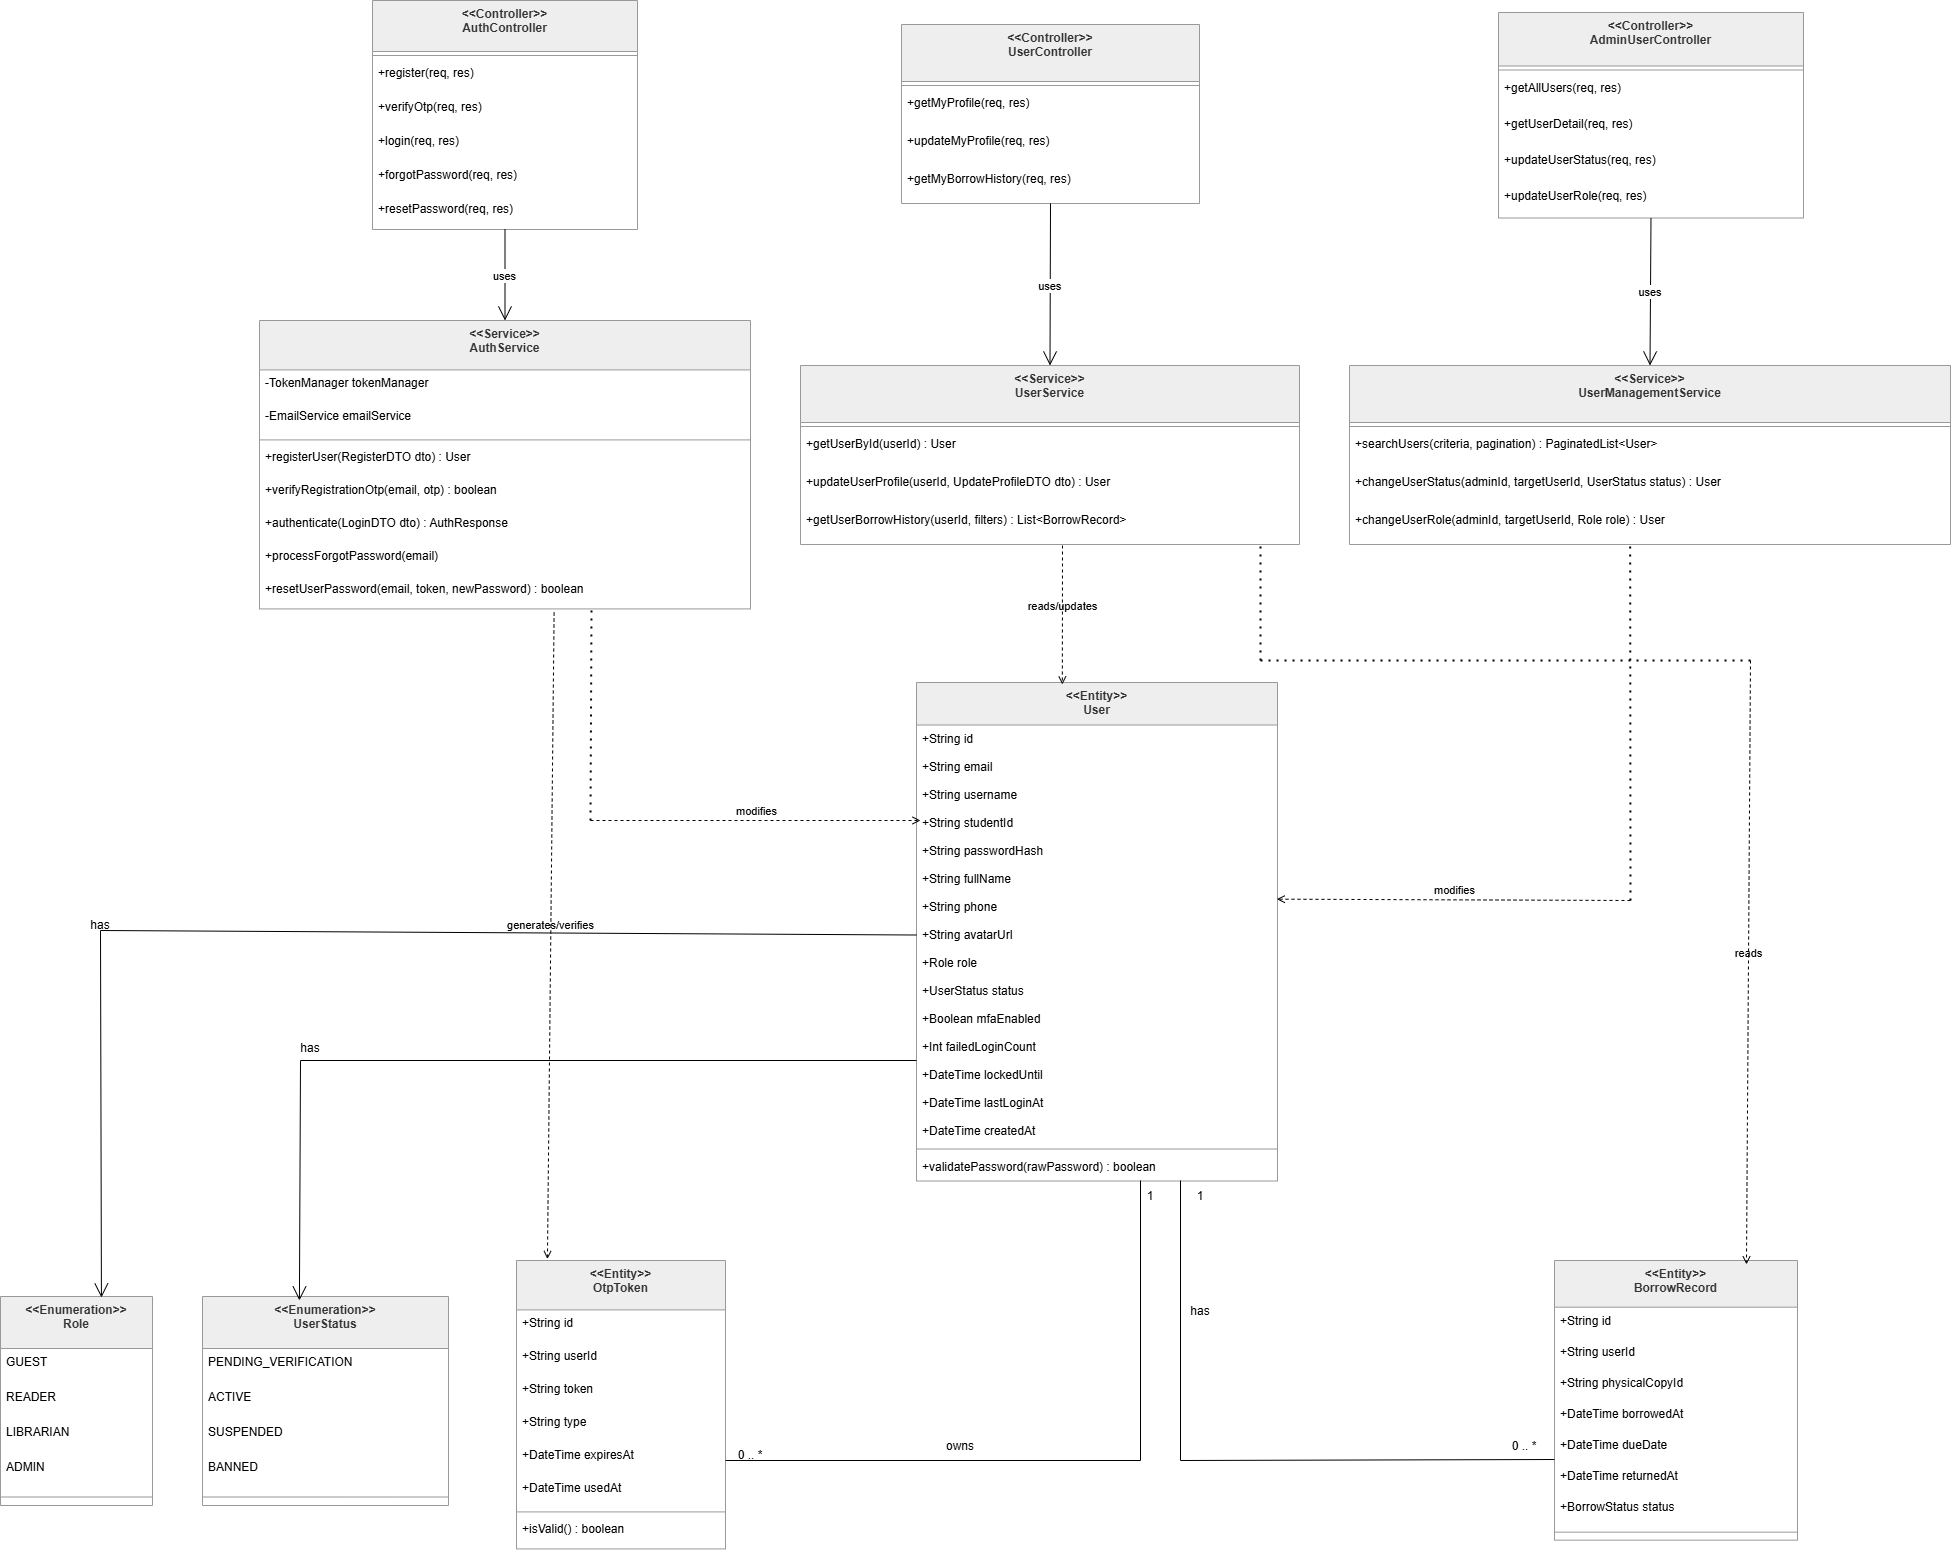
\includegraphics[width=0.6\linewidth]{Images/quanlytruycapvataikhoan.png}
	\vspace{10pt}
	\caption{Class Diagram for Account and Access Management}
	\label{fig:class_account}
\end{figure}

The \textbf{Account and Access Management} class diagram models object structures, attributes, and methods for authentication and profile management.

The central entity is \texttt{User}, containing attributes \texttt{id}, \texttt{email}, \texttt{username}, \texttt{fullName}, \texttt{phone}, \texttt{avatarUrl}, \texttt{studentId}, alongside security attributes \texttt{passwordHash}, \texttt{mfaEnabled}, \texttt{failedLoginCount}, \texttt{lockedUntil}, \texttt{lastLoginAt}, and \texttt{createdAt}. The core method \texttt{validatePassword(rawPassword)} performs credential verification.

\texttt{User} holds associations with \texttt{Role} (READER, LIBRARIAN, ADMIN) and \texttt{UserStatus} (PENDING\_VERIFICATION, ACTIVE, SUSPENDED, BANNED). \texttt{User} associates $1 - 0..*$ with \texttt{OtpToken} (method \texttt{isValid()}) and $1 - 0..*$ with \texttt{BorrowRecord}.

Architecturally, \texttt{AuthController} relies on \texttt{AuthService} (\texttt{registerUser}, \texttt{verifyRegistrationOtp}, \texttt{authenticate}, \texttt{processForgotPassword}, \texttt{resetPasswordUser}). \texttt{UserController} relies on \texttt{UserService} (\texttt{getUserById}, \texttt{updateUserProfile}, \texttt{getUserBorrowHistory}). \texttt{AdminUserController} uses \texttt{UserManagementService} (\texttt{searchUsers}, \texttt{getUserDetail}, \texttt{changeUserStatus}, \texttt{changeUserRole}).

\subsubsection{Book Catalog Management}

\begin{figure}[H]
	\centering
	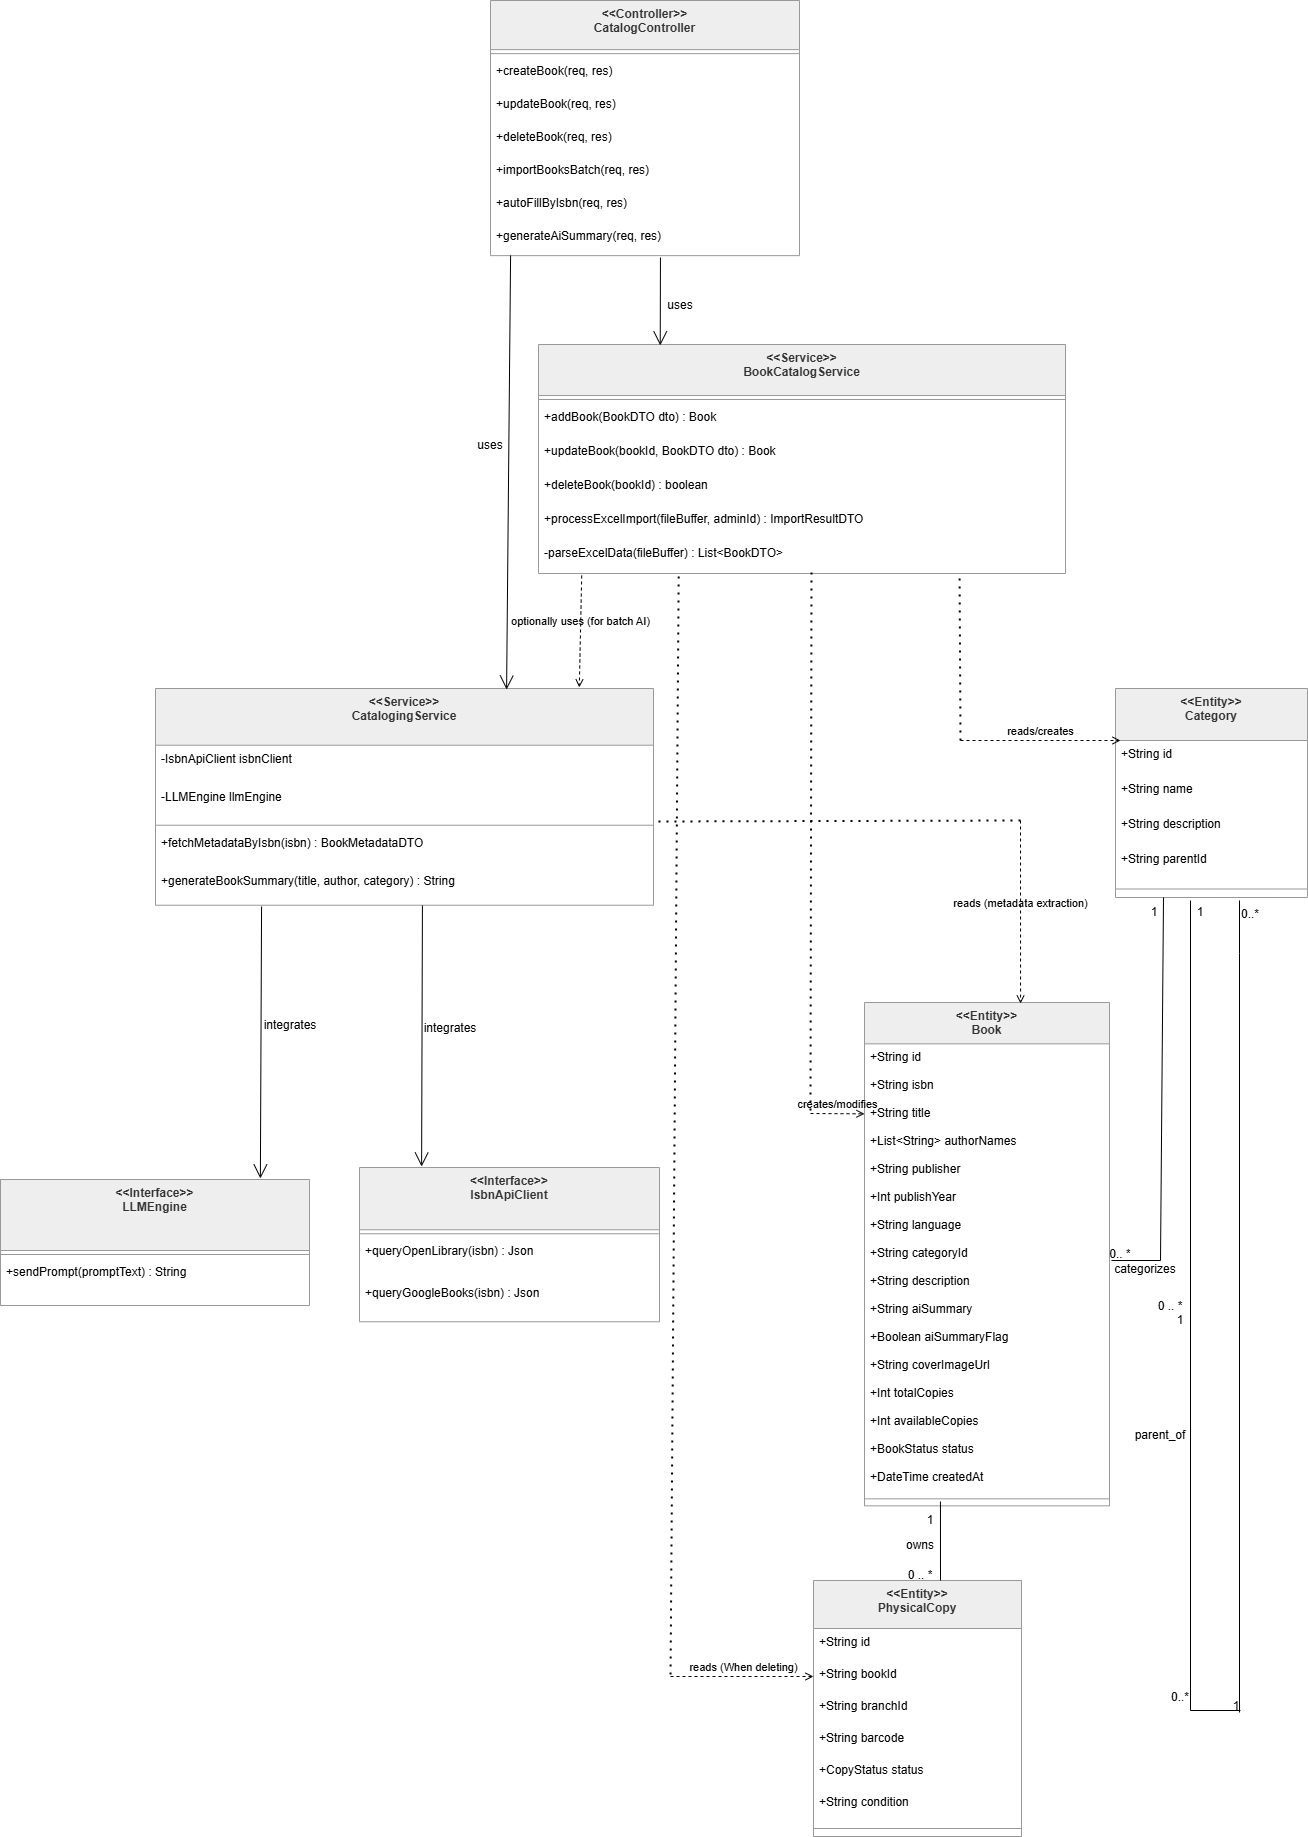
\includegraphics[width=0.6\linewidth]{Images/quanlydanhmuc.png}
	\vspace{10pt}
	\caption{Class Diagram for Book Catalog Management}
	\label{fig:class_catalog}
\end{figure}

Core data structures include \texttt{Category}, \texttt{Book}, and \texttt{PhysicalCopy}. \texttt{Category} features a self-referential hierarchy ($1 \to 0..\ast$) via \texttt{parentId} and associates $1 \to 0..\ast$ with \texttt{Book}.

\texttt{Book} holds catalog metadata (\texttt{isbn}, \texttt{title}, \texttt{authorNames}, \texttt{publisher}, \texttt{publishYear}, \texttt{language}, \texttt{totalCopies}, \texttt{availableCopies}, \texttt{aiSummary}) and associates $1 \to 0..\ast$ with \texttt{PhysicalCopy} (\texttt{barcode}, \texttt{CopyStatus status}, \texttt{condition}).

\texttt{CatalogController} delegates to \texttt{BookCatalogService} (\texttt{addBook}, \texttt{updateBook}, \texttt{deleteBook}, \texttt{autoFillByIsbn}, \texttt{generateAiSummary}, \texttt{processExcelImport}). \texttt{BookCatalogService} interacts with \texttt{CatalogingService}, which wraps \texttt{IsbnApiClient} (\texttt{queryOpenLibrary}, \texttt{queryGoogleBooks}) and \texttt{LLMEngine} (\texttt{generateBookSummary}) for automated cataloging.

\subsubsection{Document Circulation Management}

\begin{figure}[H]
	\centering
	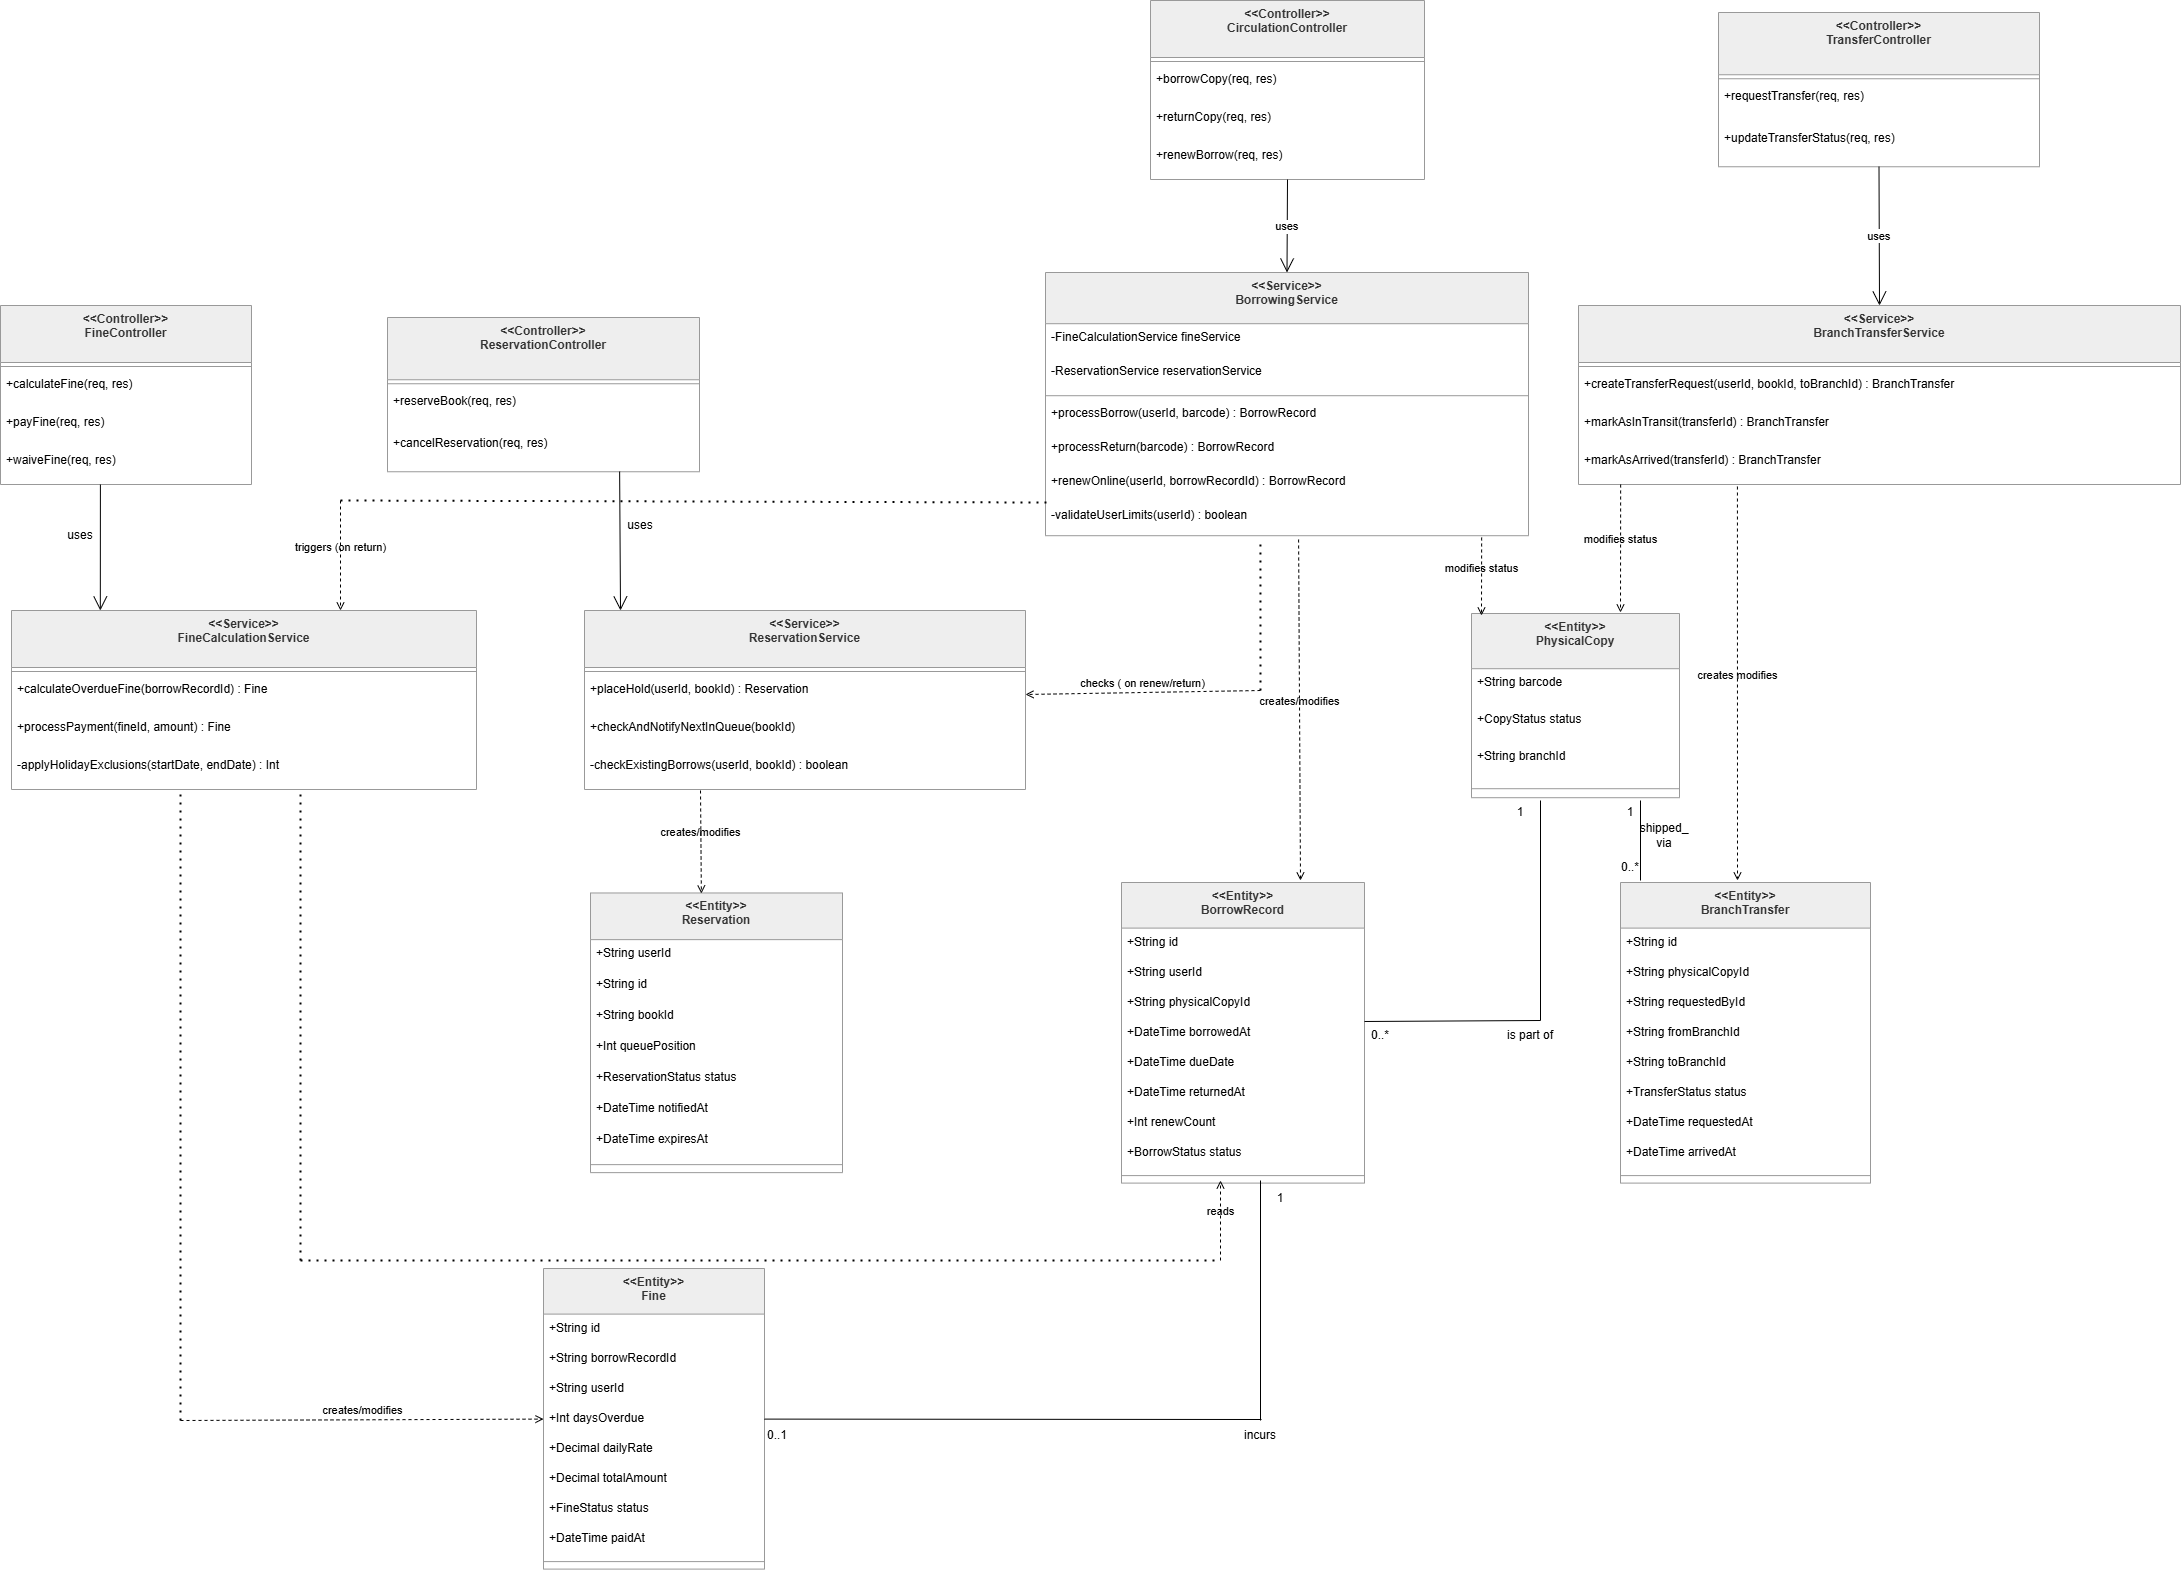
\includegraphics[width=0.6\linewidth]{Images/quanlyluuthong.png}
	\vspace{10pt}
	\caption{Class Diagram for Document Circulation Management}
	\label{fig:class_circulation}
\end{figure}

The central entity \texttt{BorrowRecord} (\texttt{borrowedAt}, \texttt{dueDate}, \texttt{returnedAt}, \texttt{renewCount}, \texttt{BorrowStatus status}) associates with \texttt{PhysicalCopy} ($1 - 0..*$). \texttt{Reservation} (\texttt{queuePosition}, \texttt{ReservationStatus status}) and \texttt{Fine} ($1 - 0..1$ with \texttt{BorrowRecord}) handle hold queues and fine assessments. \texttt{BranchTransfer} tracks inter-branch item transfers.

\texttt{CirculationController} uses \texttt{BorrowingService} (\texttt{processBorrow}, \texttt{processReturn}, \texttt{renewOnline}). \texttt{ReservationController} uses \texttt{ReservationService} (\texttt{placeHold}, \texttt{cancelReservation}). \texttt{FineController} uses \texttt{FineCalculationService} (\texttt{calculateOverdueFine}, \texttt{processPayment}). \texttt{TransferController} uses \texttt{BranchTransferService} (\texttt{createTransferRequest}, \texttt{markInTransit}, \texttt{markAsArrived}).

\subsubsection{Resource Search and Exploitation}

\begin{figure}[H]
	\centering
	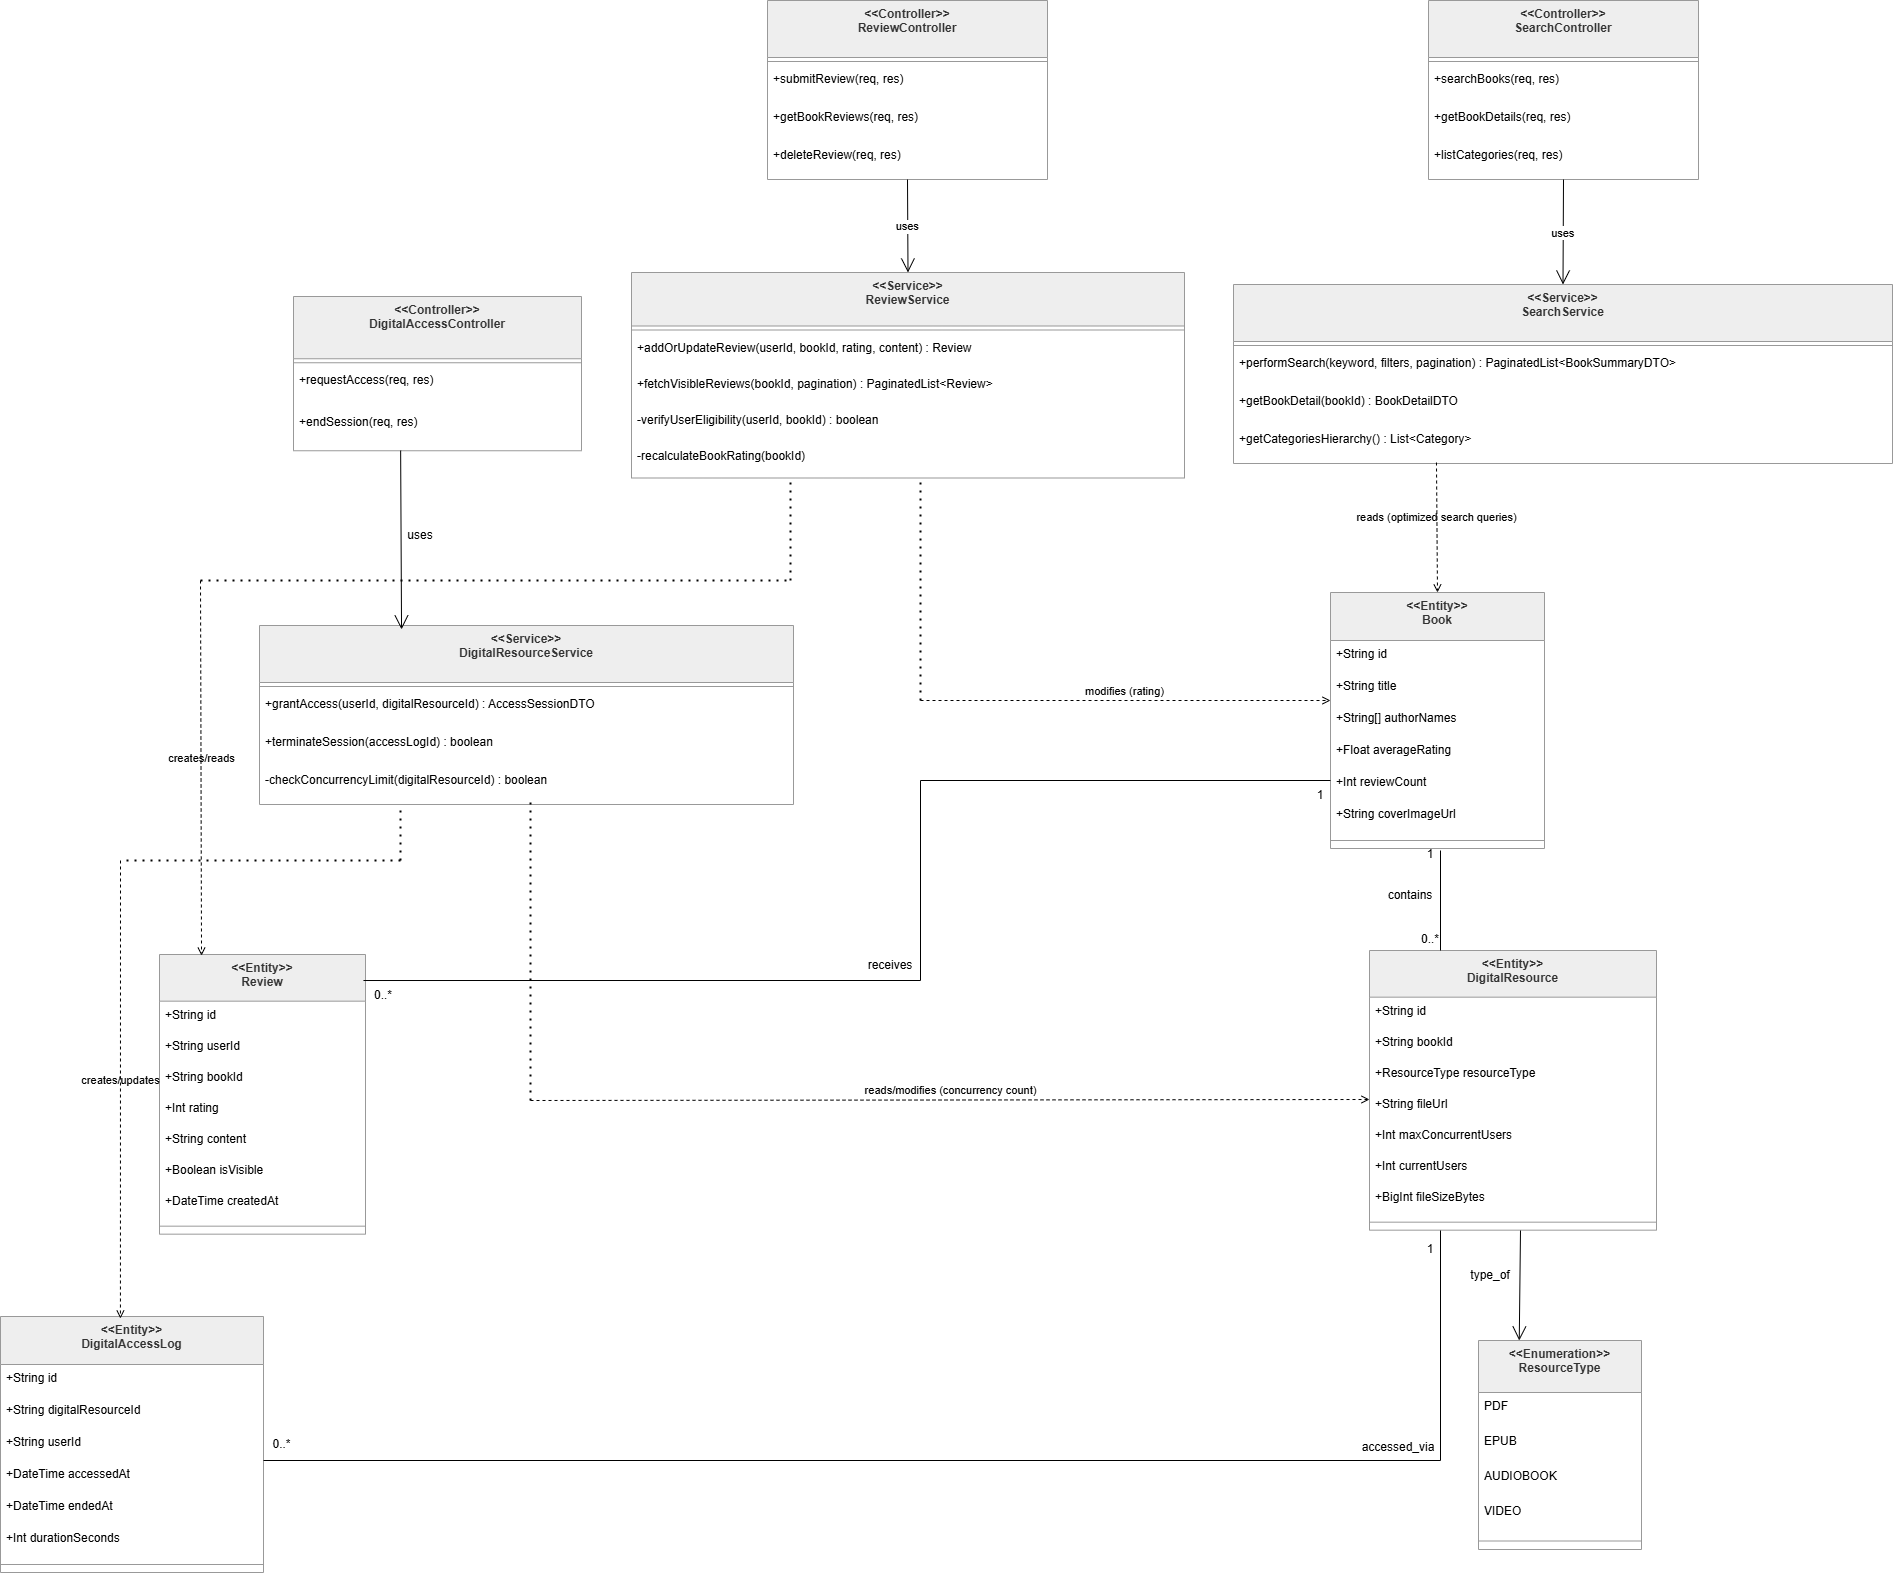
\includegraphics[width=0.6\linewidth]{Images/truycapvakhaithactainguyen.png}
	\vspace{10pt}
	\caption{Class Diagram for Resource Search and Exploitation}
	\label{fig:class_exploration}
\end{figure}

\texttt{Book} associates $1 - 0..*$ with \texttt{Review} ($0..* - 1$ with \texttt{Book}) storing user ratings.
% \texttt{Book} associates $1 - 0..*$ with \texttt{DigitalResource} (\texttt{fileUrl}, \texttt{maxConcurrentUsers}, \texttt{currentUsers}) typed by \texttt{ResourceType} (PDF, EPUB, AUDIOBOOK, VIDEO). \texttt{DigitalAccessLog} ($0..* - 1$ with \texttt{DigitalResource}) stores digital access metrics. [Not implemented in this version]

\texttt{SearchController} uses \texttt{SearchService} (\texttt{performSearch}, \texttt{getBookDetail}). \texttt{ReviewController} uses \texttt{ReviewService} (\texttt{addOrUpdateReview}, \texttt{recalculateBookRating}).
% \texttt{DigitalAccessController} uses \texttt{DigitalResourceService} (\texttt{requestAccess}, \texttt{endSession}, \texttt{checkConcurrencyLimit}). [Not implemented]

\subsubsection{AI Virtual Assistant and Recommendations}

\begin{figure}[H]
	\centering
	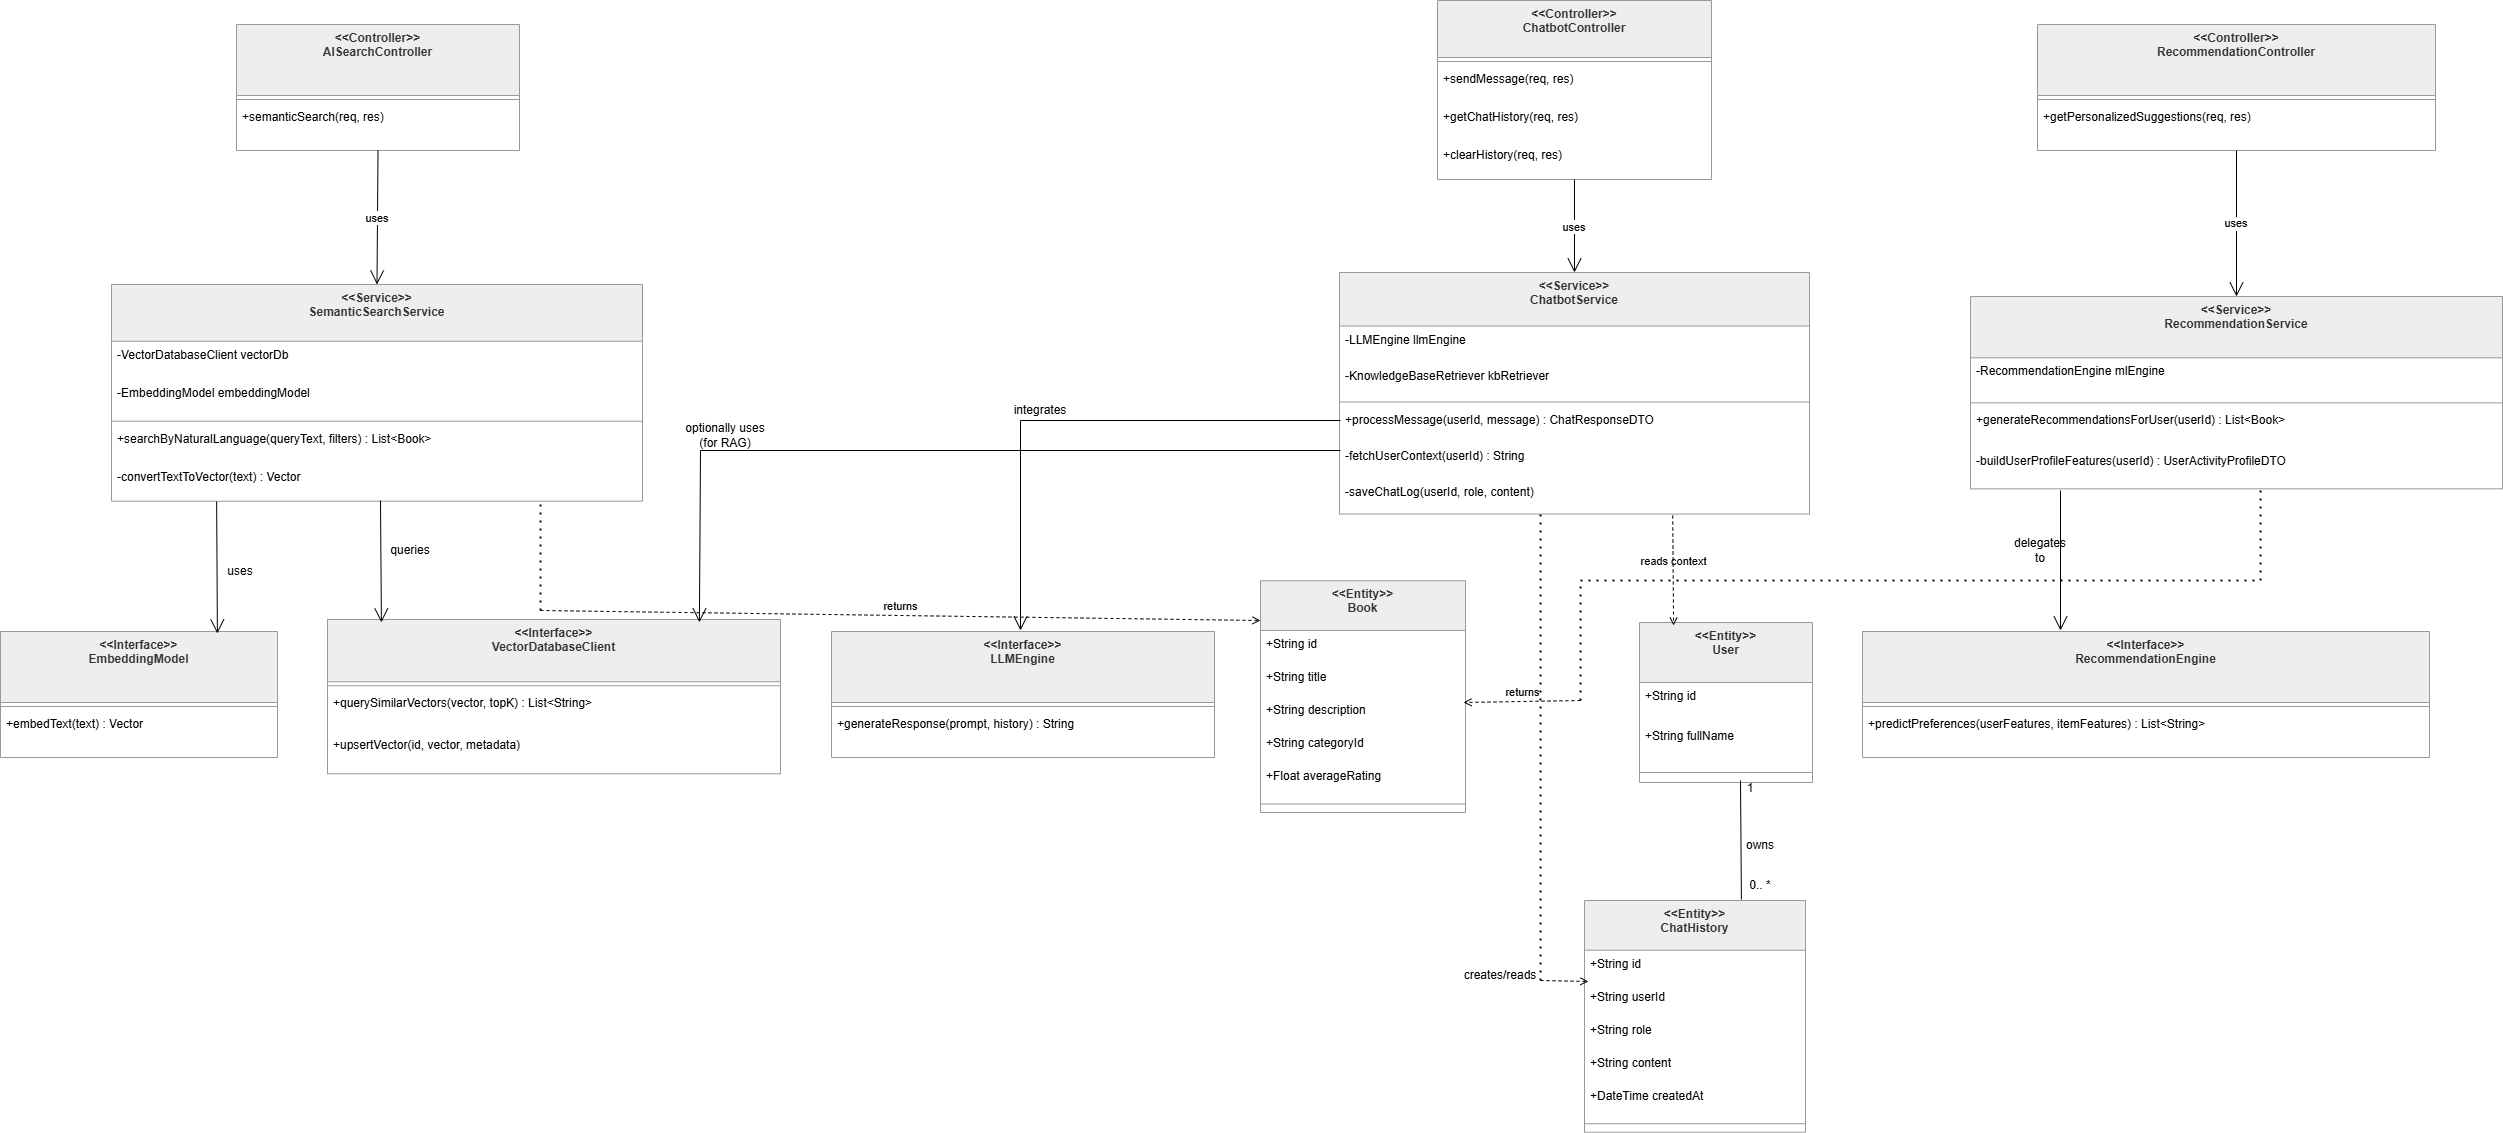
\includegraphics[width=0.6\linewidth]{Images/AI.png}
	\vspace{10pt}
	\caption{Class Diagram for AI Virtual Assistant and Recommendations}
	\label{fig:class_ai}
\end{figure}

\texttt{AISearchController} uses \texttt{SemanticSearchService} (\texttt{searchByNaturalLanguage}) interfacing with \texttt{EmbeddingModel} and \texttt{VectorDatabaseClient}.

\texttt{ChatbotController} uses \texttt{ChatbotService} (\texttt{sendMessage}, \texttt{getChatHistory}), interfacing with \texttt{LLMEngine} and \texttt{VectorDatabaseClient} (RAG context), logging chats in \texttt{ChatHistory}.

\texttt{RecommendationController} uses \texttt{RecommendationService} (\texttt{getPersonalizedSuggestions}), leveraging \texttt{RecommendationEngine} (\texttt{predictPreferences}) to return tailored book lists.

\subsubsection{Notifications and Communication}

\begin{figure}[H]
	\centering
	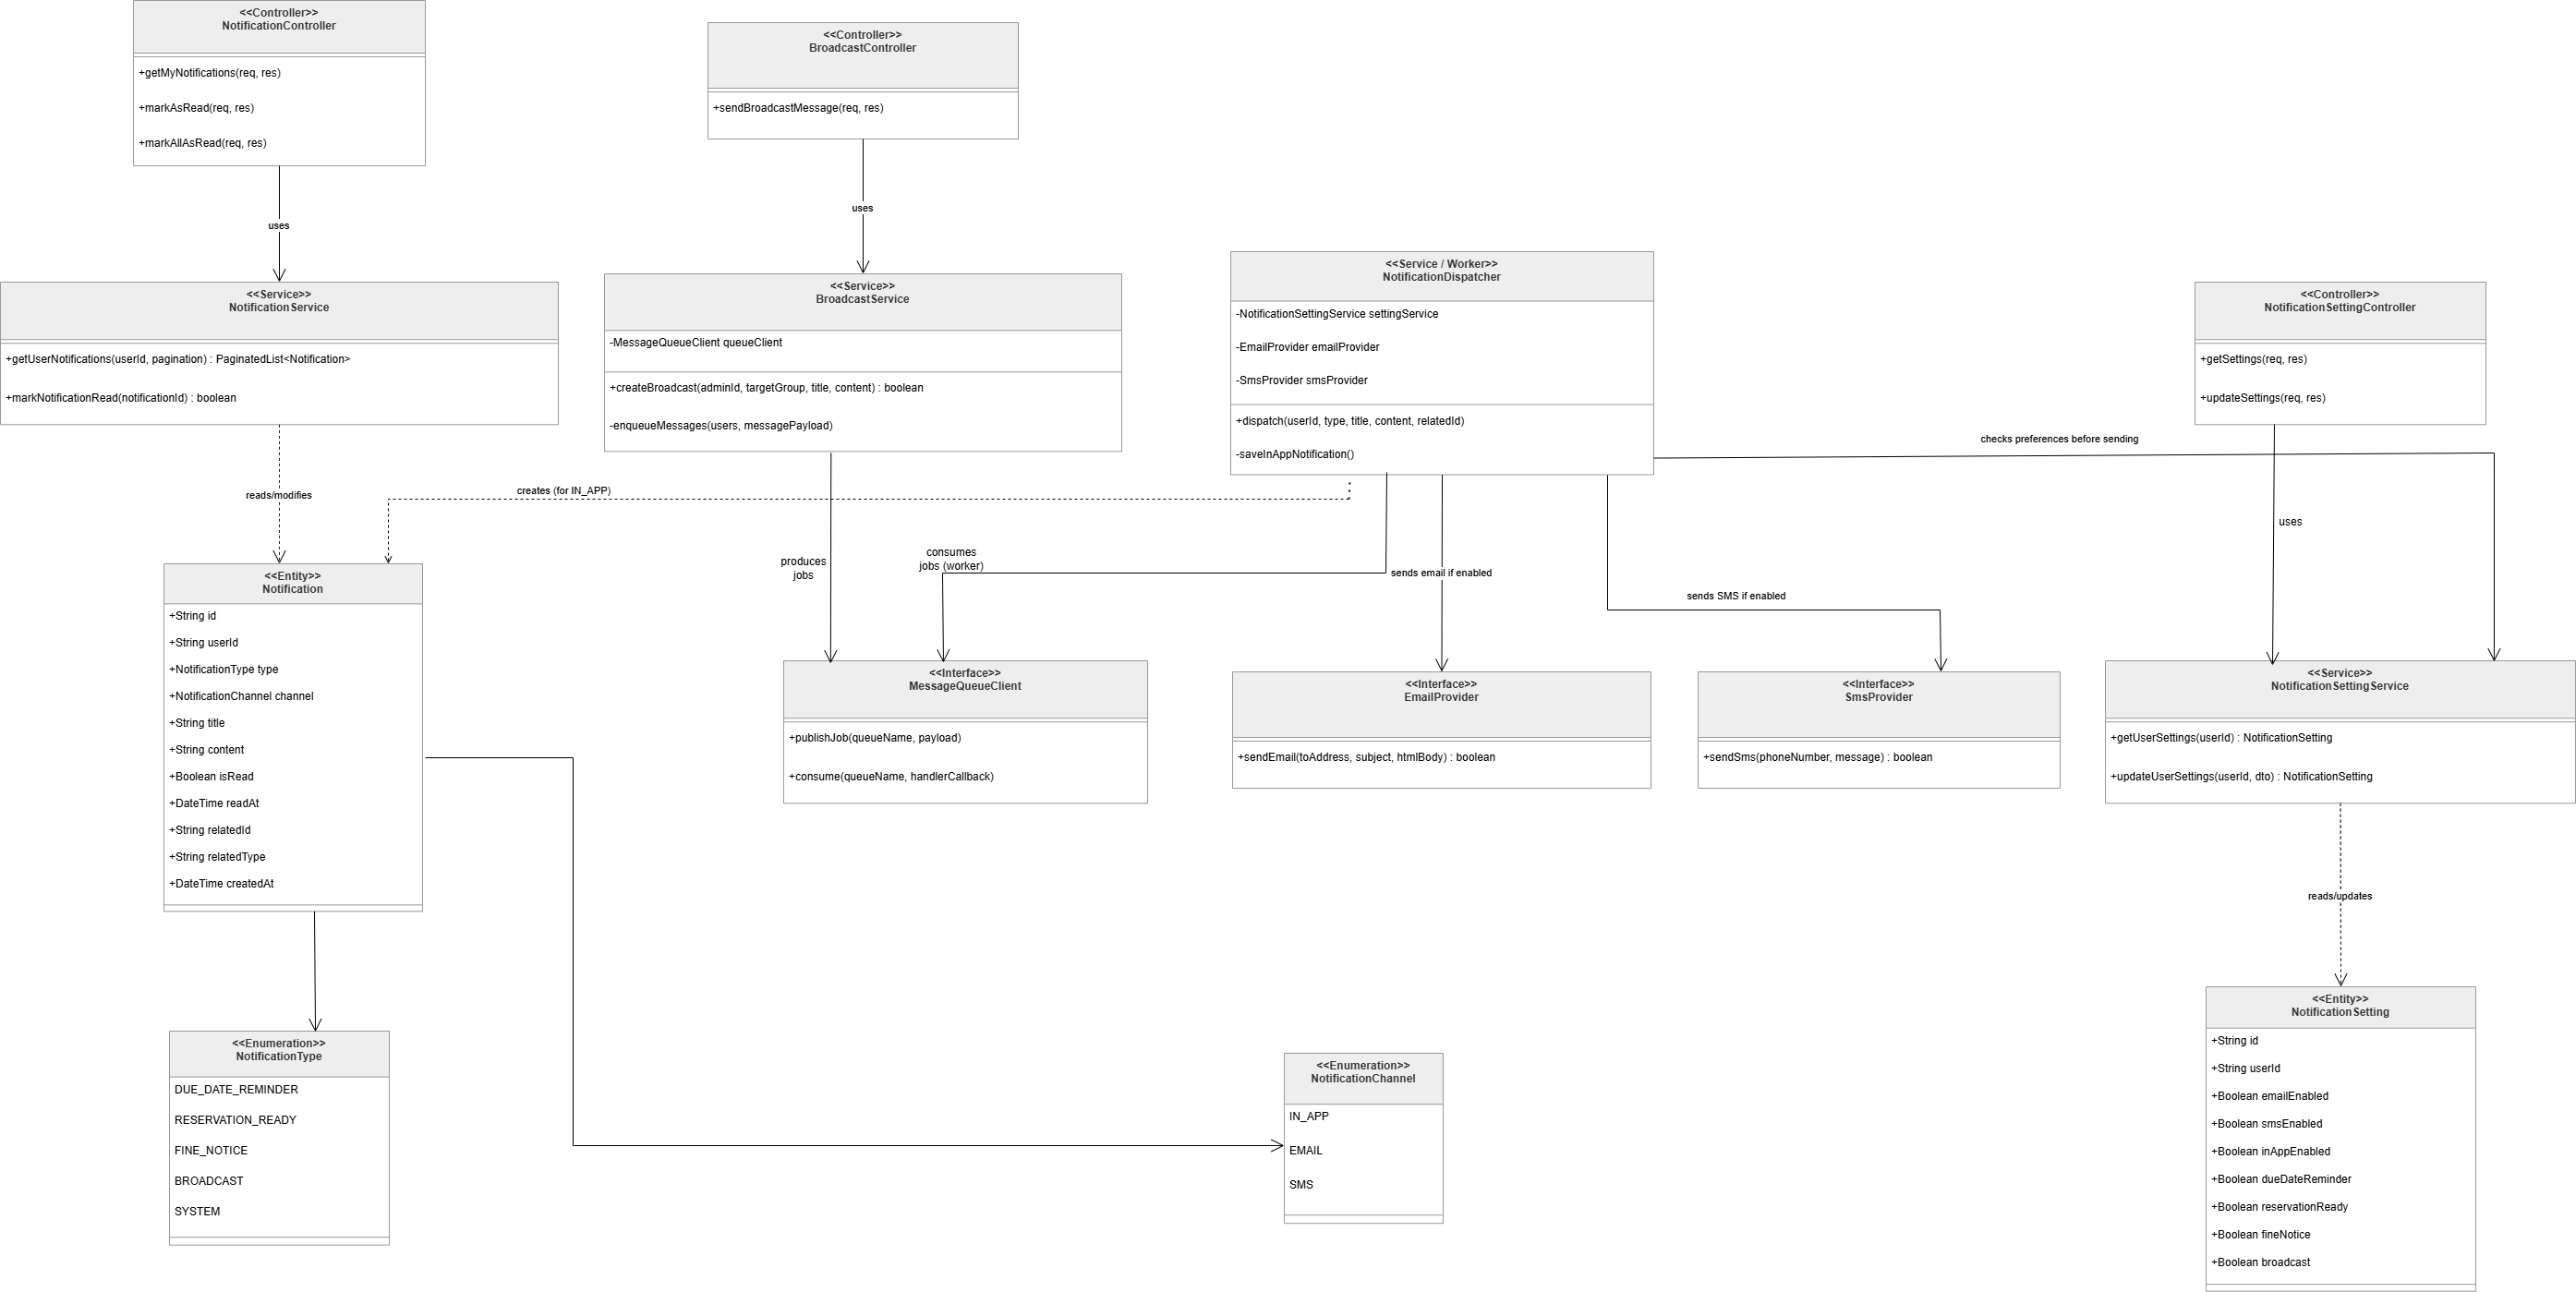
\includegraphics[width=0.6\linewidth]{Images/thongbao.png}
	\vspace{10pt}
	\caption{Class Diagram for Notifications and Communication}
	\label{fig:class_notification}
\end{figure}

Entities comprise \texttt{Notification} (\texttt{isRead}, \texttt{NotificationType}, \texttt{NotificationChannel}) and \texttt{NotificationSetting} (\texttt{emailEnabled}, \texttt{smsEnabled}, \texttt{inAppEnabled}).

\texttt{NotificationSettingController} uses \texttt{NotificationSettingService}. \texttt{NotificationController} uses \texttt{NotificationService}. \texttt{BroadcastController} uses \texttt{BroadcastService} pushing jobs to \texttt{MessageQueueClient}. Async worker \texttt{NotificationDispatcher} consumes queue jobs and dispatches alerts via \texttt{EmailProvider} and \texttt{SmsProvider}.

\subsubsection{System Administration}

\begin{figure}[H]
	\centering
	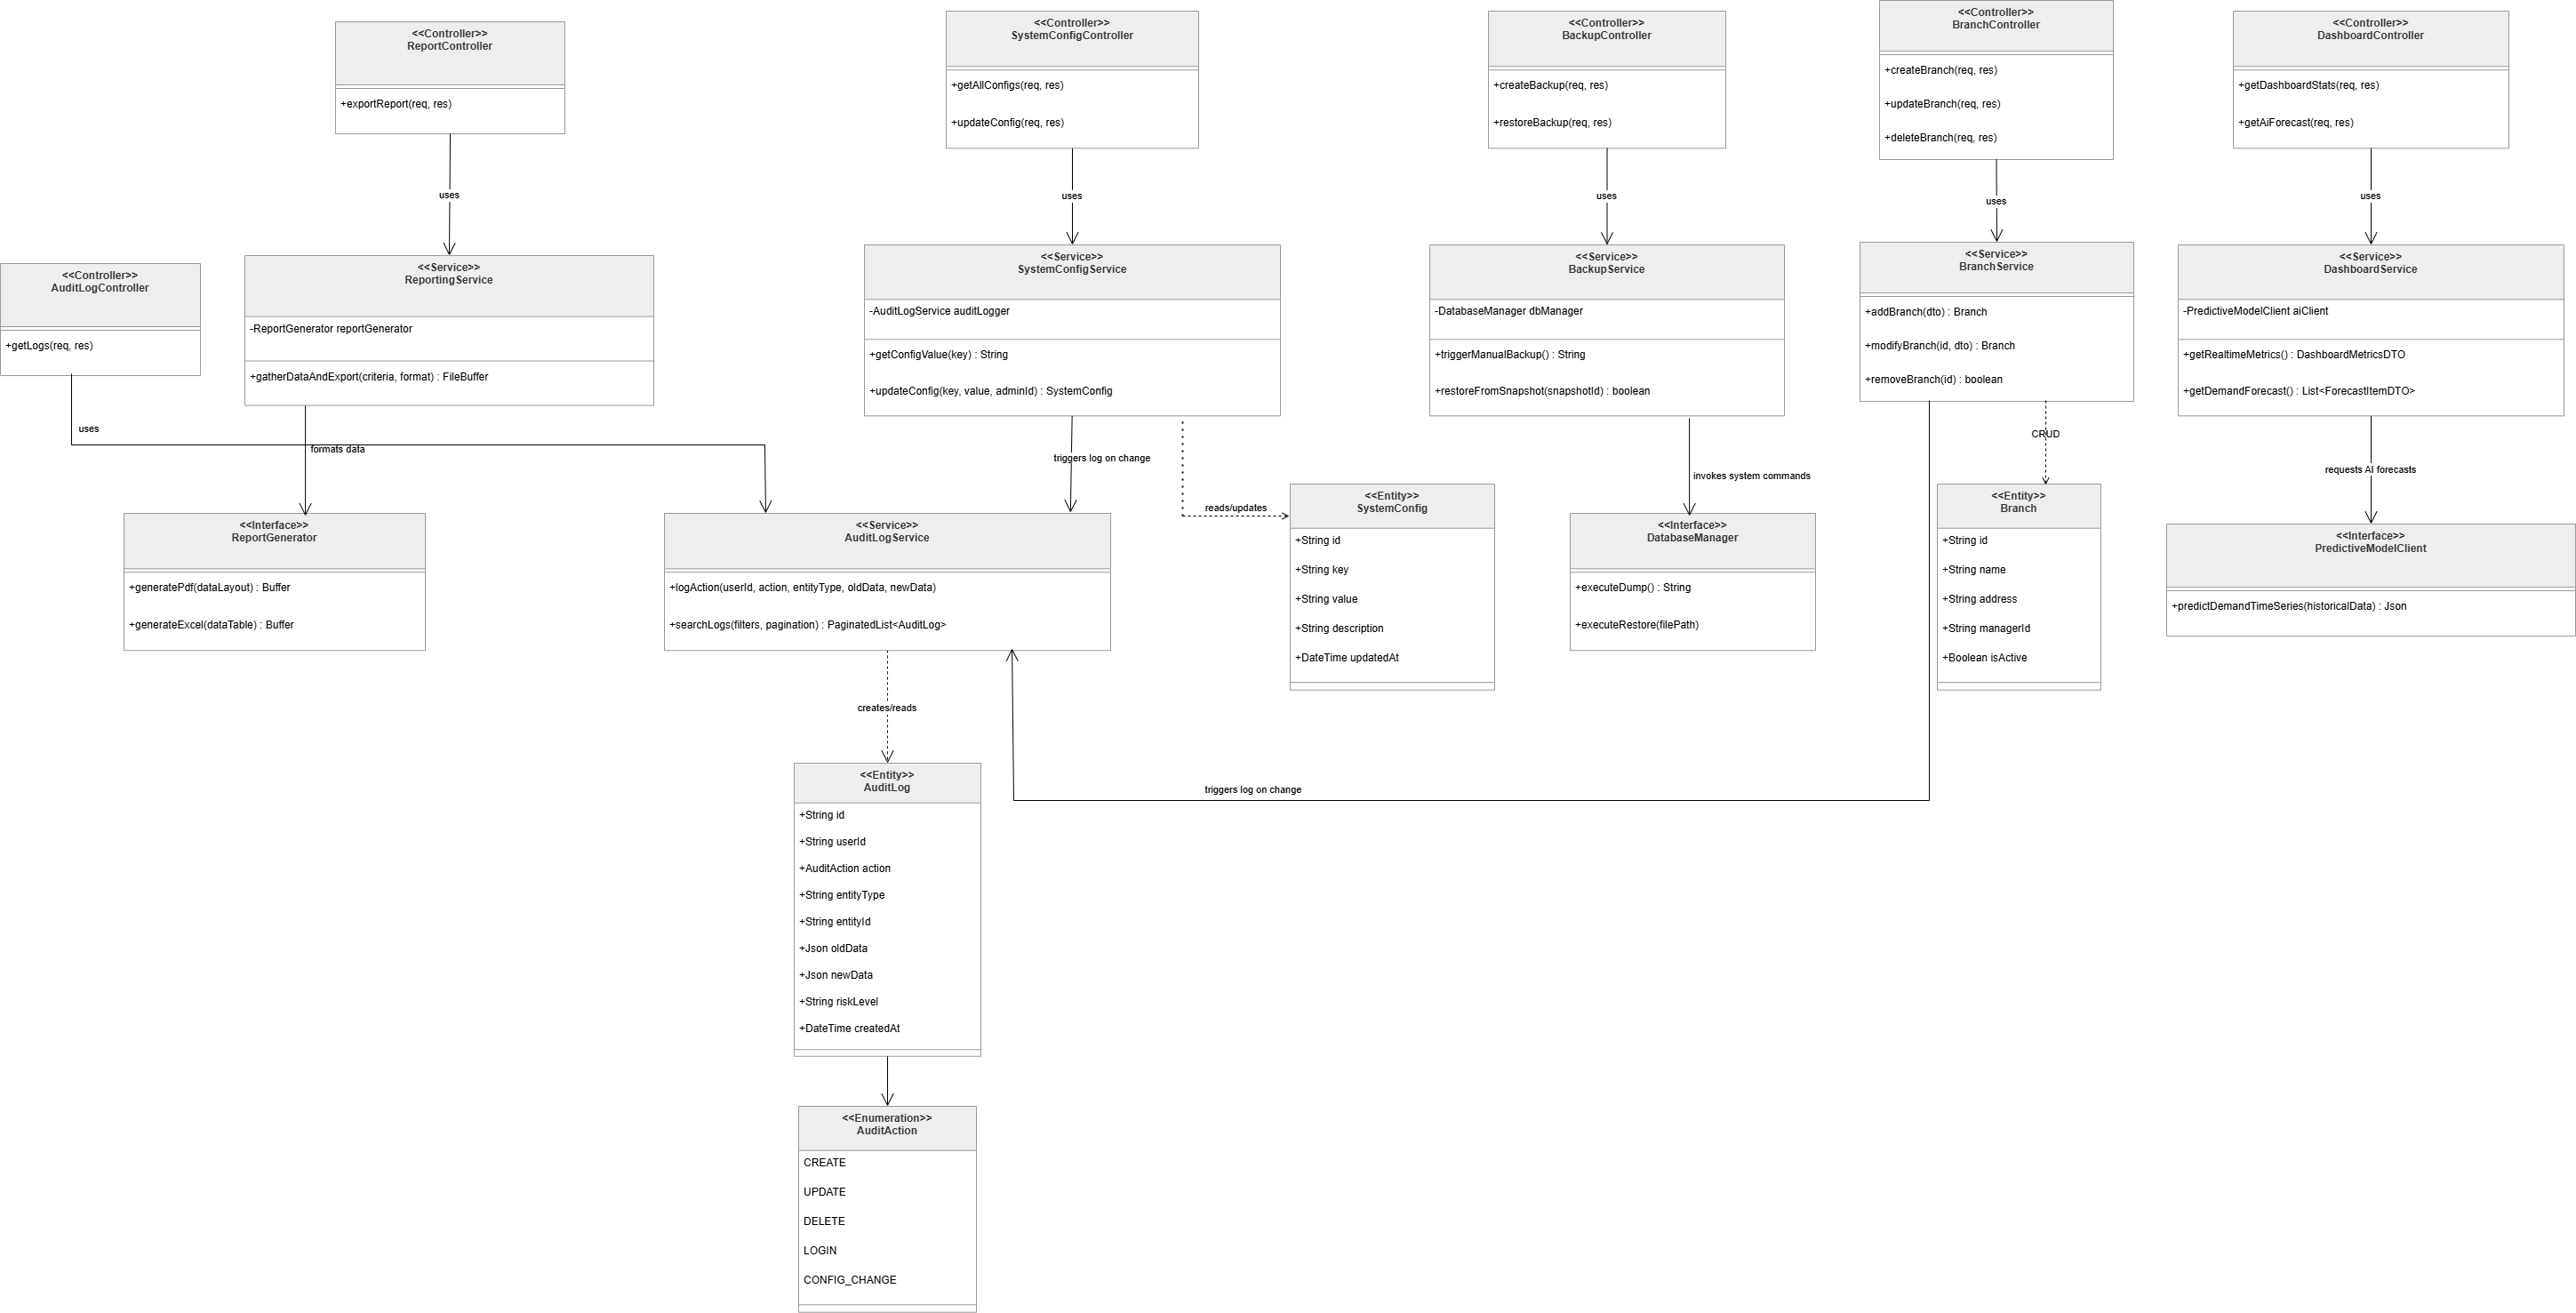
\includegraphics[width=0.6\linewidth]{Images/baocaovaquantri.png}
	\vspace{10pt}
	\caption{Class Diagram for System Administration}
	\label{fig:class_admin}
\end{figure}

Core entities: \texttt{AuditLog} (\texttt{action}, \texttt{oldData}, \texttt{newData}, \texttt{riskLevel}), \texttt{SystemConfig} (\texttt{key}, \texttt{value}), and \texttt{Branch} (\texttt{name}, \texttt{address}, \texttt{isActive}).

\texttt{AuditLogController} uses \texttt{AuditLogService}. \texttt{ReportController} uses \texttt{ReportingService} (\texttt{ReportGenerator}). \texttt{SystemConfigController} uses \texttt{SystemConfigService}. \texttt{BackupController} uses \texttt{BackupService} (\texttt{DatabaseManager}). \texttt{BranchController} uses \texttt{BranchService}. \texttt{DashboardController} uses \texttt{DashboardService} interfacing with \texttt{PredictiveModelClient} for demand forecasting.

\subsection{Activity Diagrams}

\subsubsection{Account Registration}

The Account Registration activity diagram illustrates the end-to-end operational workflow when a new guest user creates an account in the system. This process ensures that user inputs comply with system validation rules, prevents duplicate identity registration via unique email/phone checks, and guarantees secure user verification through Multi-Factor Authentication (OTP/Activation links) before activating the profile.

\begin{figure}[H]
	\centering
	
\includegraphics[width=0.6\linewidth]{Images/dangki.png}
	\vspace{10pt}
	\caption{Activity Diagram for Account Registration}
	\label{fig:activity_register}
\end{figure}

\begin{enumerate}
	\item Guest accesses the account registration page.
	\item System displays registration form.
	\item Guest enters credentials (Full Name, Email/Phone, Password).
	\item System validates input data syntax.
	\item System checks if Email/Phone exists in database.
	\item \textbf{Valid Branch:}
	      \begin{itemize}
		      \item If valid, system sends Email/SMS containing OTP code or activation link.
		      \item Guest enters OTP code or clicks activation link.
		      \item System validates OTP code or link token.
		      \item If OTP/link is valid: System creates user account, saves to DB, sets status to "Activated", and alerts success.
	      \end{itemize}
	\item \textbf{Invalid Branch:}
	      \begin{itemize}
		      \item If data is invalid or Email/Phone exists: System displays error alert and prompts re-entry.
		      \item If OTP is invalid: System displays invalid OTP error and cancels registration session.
	      \end{itemize}
\end{enumerate}

\subsubsection{System Login}

The System Login activity diagram depicts the authentication sequence for existing users accessing the system. It handles identity verification against stored credentials and incorporates adaptive security controls—such as mandatory Multi-Factor Authentication (MFA) and automated temporary account lockouts after multiple failed attempts—to protect the platform against brute-force attacks.

\begin{figure}[H]
	\centering
	
\includegraphics[width=0.6\linewidth]{Images/dangnhap.png}
	\vspace{10pt}
	\caption{Activity Diagram for System Login}
	\label{fig:activity_login}
\end{figure}

\begin{enumerate}
	\item User accesses login view.
	\item User enters Email/Username and Password.
	\item System validates credentials against DB.
	\item If credentials invalid: System displays error "Incorrect account or password".
	\item If credentials valid: System checks if Multi-Factor Authentication (MFA) is required.
	\item If MFA enabled: System requests OTP code; user enters OTP; system validates code.
	\item If OTP invalid: Displays error "Incorrect OTP code". If failed attempts > 3, account is temporarily locked for 15 minutes.
	\item If OTP valid (or MFA not required): Initializes session/token, redirects user to role dashboard, and displays success notification.
\end{enumerate}

\subsubsection{Password Reset}

The Password Reset activity diagram outlines the self-service credential recovery mechanism for users who have forgotten their passwords. The workflow relies on secure, time-sensitive verification tokens sent directly to the user's registered email address, ensuring that password updates occur safely without administrator intervention.

\begin{figure}[H]
	\centering
	
\includegraphics[width=0.6\linewidth]{Images/datlai.png}
	\vspace{10pt}
	\caption{Activity Diagram for Password Reset}
	\label{fig:activity_reset_password}
\end{figure}

\begin{enumerate}
	\item User selects "Forgot Password".
	\item System prompts for Email.
	\item User submits Email.
	\item System verifies Email existence. If not found: Display "No account found with this email".
	\item If found: System sends reset link via Email. User opens link; system verifies token validity.
	\item If link expired/invalid: Display "Reset link expired" and prompt process restart.
	\item If link valid: Display reset form; user enters new password; system hashes and updates password, alerting success.
\end{enumerate}

\subsubsection{View Loan/Return History}

The View Loan/Return History activity diagram models how users query and inspect their personal borrowing records over time. It demonstrates the interactions involved in fetching structured loan logs from the persistent database and allowing users to dynamically filter results based on execution dates or current item statuses (e.g., Active, Returned, Overdue).

\begin{figure}[H]
	\centering
	
\includegraphics[width=0.6\linewidth]{Images/xemlichsu.png}
	\vspace{10pt}
	\caption{Activity Diagram for View Loan/Return History}
	\label{fig:activity_view_history}
\end{figure}

\begin{enumerate}
	\item User logs into system.
	\item User opens "Borrowing History" on dashboard.
	\item System queries DB for loan records matching User ID.
	\item System renders loan history table (Title, Borrow Date, Due Date, Return Date, Status, Fines).
	\item User can apply filters by date range or status.
	\item System refreshes table view based on applied filter parameters.
\end{enumerate}

\subsubsection{User Account Management}

The User Account Management activity diagram presents the administrative control workflow for managing user accounts system-wide. Authorized System Administrators can search, review, create, edit, lock/unlock, or adjust role permissions (Role-Based Access Control) for any user profile while maintaining overall access compliance.

\begin{figure}[H]
	\centering
	
\includegraphics[width=0.6\linewidth]{Images/quanly.png}
	\vspace{10pt}
	\caption{Activity Diagram for User Account Management}
	\label{fig:activity_manage_users}
\end{figure}

\begin{enumerate}
	\item Admin logs in and accesses "User Management".
	\item System renders user list (ID, Name, Email, Role, Status).
	\item Admin selects a target user and an operation (Add User, Edit Profile, Delete User, Toggle Status, Change Role).
	\item Executes selected workflow; system validates input data and updates DB, displaying success confirmation upon completion.
\end{enumerate}

\subsubsection{Add / Edit / Delete Catalog Record}

This activity diagram describes the cataloging management actions performed by Librarians to keep the library database accurate. It handles single-item entries, updates, and soft deletions, including validation checks to prevent the deletion of items currently actively checked out by patrons.

\begin{figure}[H]
	\centering
	
\includegraphics[width=0.6\linewidth]{Images/edit.png}
	\vspace{10pt}
	\caption{Activity Diagram for Add / Edit / Delete Catalog Record}
	\label{fig:activity_manage_documents}
\end{figure}

\begin{enumerate}
	\item Librarian opens "Catalog Management".
	\item Librarian selects action: Add, Edit, or Delete.
	\item If Delete: System verifies active loans. If item is checked out, deletion is blocked ("Cannot delete: Item checked out"). Otherwise, soft delete is performed.
	\item If Add/Edit: Form is rendered; optional ISBN auto-cataloging (UC-CAT-03) or AI summary generation (UC-CAT-04) can be triggered.
	\item System validates fields, persists updates, and alerts success.
\end{enumerate}

\subsubsection{Batch Catalog Data Ingestion}

The Batch Catalog Data Ingestion activity diagram details the process of importing bulk book catalog data into the system using external files (CSV/Excel). The workflow highlights parsing, pre-import validation, error logging for malformed records, and database transaction execution to facilitate rapid catalog updates.

\begin{figure}[H]
	\centering
	
\includegraphics[width=0.6\linewidth]{Images/nhap.png}
	\vspace{10pt}
	\caption{Activity Diagram for Batch Catalog Data Ingestion}
	\label{fig:activity_import}
\end{figure}

\begin{enumerate}
	\item Librarian selects "Batch Import".
	\item Uploads catalog data file (CSV/Excel).
	\item System parses file and displays preview table with valid/invalid record counts.
	\item Librarian confirms import execution.
	\item System writes valid rows to DB and reports results. If errors exist, librarian can fix file and re-upload or cancel operation.
\end{enumerate}

\subsubsection{Automated Cataloging via ISBN}

The Automated Cataloging via ISBN activity diagram depicts how the system integrates with external metadata services (Google Books API, Open Library API). Librarians provide an ISBN code, and the system automatically queries external APIs to populate book metadata fields, reducing manual data entry overhead.

\begin{figure}[H]
	\centering
	
\includegraphics[width=0.6\linewidth]{Images/bienmuc.png}
	\vspace{10pt}
	\caption{Activity Diagram for Automated Cataloging via ISBN}
	\label{fig:activity_isbn}
\end{figure}

\begin{enumerate}
	\item Librarian enters ISBN.
	\item System sends API request to external sources (Google Books, Open Library).
	\item Parses JSON response and populates form fields.
	\item Librarian reviews and saves catalog record. If ISBN is not found, librarian switches to manual data entry.
\end{enumerate}

\subsubsection{Physical Material Checkout}

The Physical Material Checkout activity diagram specifies the desk circulation process when a reader borrows physical books. It captures barcode scanning operations, verifies reader eligibility (account status, unpaid fine limits, max loan allowances), updates item copy availability, and registers checkout records.

\begin{figure}[H]
	\centering
	
\includegraphics[width=0.6\linewidth]{Images/muon.png}
	\vspace{10pt}
	\caption{Activity Diagram for Physical Material Checkout}
	\label{fig:activity_borrow}
\end{figure}

\begin{enumerate}
	\item Librarian logs in and scans Reader card barcode.
	\item System verifies reader account status and fine balance.
	\item If eligible, librarian scans item barcodes.
	\item System checks loan limits per role and hold queue restrictions.
	\item Creates loan record, calculates due date, updates copy status to "Checked Out", and decrements inventory count.
\end{enumerate}

\subsubsection{Material Return}

The Material Return activity diagram details the operational flow executed when physical books are returned to the library desk. The system closes the active borrow record, evaluates potential overdue days to initiate fine calculation workflows if necessary, and inspects reservation queues to transition the copy state appropriately.

\begin{figure}[H]
	\centering
	
\includegraphics[width=0.6\linewidth]{Images/tra.png}
	\vspace{10pt}
	\caption{Activity Diagram for Material Return}
	\label{fig:activity_return}
\end{figure}

\begin{enumerate}
	\item Librarian scans returned item barcode.
	\item System retrieves loan record and checks due date.
	\item If overdue, triggers fine assessment workflow (UC-CIR-03).
	\item Sets loan status to "Completed".
	\item Checks reservation queue: if hold exists, sets copy to "Awaiting Pickup" and alerts next user; if no hold, sets copy to "Available".
\end{enumerate}

\subsubsection{Calculate and Assess Overdue Fines}

The Calculate and Assess Overdue Fines activity diagram models the financial penalty workflow for items returned after their due dates. The system automatically computes overdue durations (excluding official library holidays), applies daily penalty rates, and posts the resulting fine balance to the reader's account or processes immediate payment receipts.

\begin{figure}[H]
	\centering
	
\includegraphics[width=0.5\linewidth]{Images/phiphat.png}
	\vspace{10pt}
	\caption{Activity Diagram for Calculate and Assess Overdue Fines}
	\label{fig:activity_fine}
\end{figure}

\begin{enumerate}
	\item System computes overdue days (Return Date - Due Date), excluding library holidays.
	\item Multiplies overdue days by daily fine rate.
	\item Renders fine calculation. If reader pays immediately, generates receipt and sets ledger balance to 0; otherwise posts fine balance to reader account ledger.
\end{enumerate}

\subsubsection{Online Loan Renewal}

The Online Loan Renewal activity diagram presents the self-service capability that allows readers to extend their borrowing period over the web. The system validates renewal constraints—such as ensuring maximum allowed renewals haven't been exceeded and checking that no other patron has placed a hold reservation on the item.

\begin{figure}[H]
	\centering
	
\includegraphics[width=0.6\linewidth]{Images/giahan.png}
	\vspace{10pt}
	\caption{Activity Diagram for Online Loan Renewal}
	\label{fig:activity_extend}
\end{figure}

\begin{enumerate}
	\item Reader opens active loans and clicks "Renew".
	\item System verifies: maximum renewal count not reached and no hold requests exist.
	\item If eligible, extends due date, increments renewal count, and displays new due date.
\end{enumerate}

\subsubsection{Place Item Hold}

The Place Item Hold activity diagram presents the reservation process when a requested material is currently out of stock. The system verifies that the user does not currently hold an active copy of the item and assigns them a sequential queue position for automated pickup notification when a copy is returned.

\begin{figure}[H]
	\centering
	
\includegraphics[width=0.5\linewidth]{Images/dat.png}
	\vspace{10pt}
	\caption{Activity Diagram for Place Item Hold}
	\label{fig:activity_reserve}
\end{figure}

\begin{enumerate}
	\item Reader opens item page and clicks "Place Hold".
	\item System verifies reader does not currently hold active loan for item and item is out of stock.
	\item System appends reader to reservation queue and displays queue position.
\end{enumerate}

\subsubsection{Document Catalog Search}

The Document Catalog Search activity diagram models how users explore the library catalog. It depicts keyword query submission, indexed database querying, paginated search result rendering, and navigation to detailed document view pages.

\begin{figure}[H]
	\centering
	
\includegraphics[width=0.6\linewidth]{Images/tracuu.png}
	\vspace{10pt}
	\caption{Activity Diagram for Document Catalog Search}
	\label{fig:activity_search}
\end{figure}

\begin{enumerate}
	\item Reader enters query keywords and selects search criteria.
	\item System queries catalog DB indexes and returns paginated results.
	\item Displays book cards. Reader clicks book card to view detail page.
\end{enumerate}

\subsection{Sequence Diagrams}

\subsubsection{Account Registration}

The Account Registration sequence diagram illustrates the step-by-step object interactions between the Reader interface, Authentication Controller, User Service, Notification Dispatcher, and Database. It details how user inputs are validated, how OTP verification tokens are dispatched asynchronously, and how the database transaction completes account activation upon successful code validation.

\begin{figure}[H]
	\centering
	
\includegraphics[width=0.6\linewidth]{Images/Seq_Dang ky.png}
	\vspace{10pt}
	\caption{Sequence Diagram for Account Registration}
	\label{fig:sequence_register}
\end{figure}

\begin{enumerate}
	\item Reader accesses registration view.
	\item Submits details; system validates inputs and checks for duplicates.
	\item System sends OTP code via email/SMS.
	\item Reader enters OTP. If OTP valid, account is created and activated; otherwise registration is canceled.
\end{enumerate}

\subsubsection{Account Login}

The Account Login sequence diagram outlines the interactive messages passed between the User Interface, Authentication Controller, Security Service, and Database during authentication. It captures credential validation, role and status verification, Multi-Factor Authentication (MFA) evaluation, and the final issuance of a JSON Web Token (JWT) session upon authorization.

\begin{figure}[H]
	\centering
	
\includegraphics[width=0.6\linewidth]{Images/Seq_Dang nhap.png}
	\vspace{10pt}
	\caption{Sequence Diagram for Account Login}
	\label{fig:sequence_login}
\end{figure}

\begin{enumerate}
	\item User submits credentials.
	\item System matches credentials against DB.
	\item If MFA enabled, requests OTP; upon successful OTP verification, issues session JWT token and redirects user to role dashboard.
\end{enumerate}

\subsubsection{Account Password Reset}

The Account Password Reset sequence diagram specifies the system interactions during a self-service credential recovery flow. It demonstrates how the system validates user identity via email lookup, generates temporary reset tokens, dispatches secure email links, and executes hashed password updates upon token verification.

\begin{figure}[H]
	\centering
	
\includegraphics[width=0.6\linewidth]{Images/Seq_Reset mat khau.png}
	\vspace{10pt}
	\caption{Sequence Diagram for Account Password Reset}
	\label{fig:sequence_reset_password}
\end{figure}

\begin{enumerate}
	\item User requests password reset by entering registered email.
	\item System verifies email, generates reset token, and dispatches reset link via email.
	\item User opens link; system verifies token validity. User submits new password; system updates password hash.
\end{enumerate}

\subsubsection{Document Search}

The Document Search sequence diagram describes the message flow initiated when a user queries the catalog. It depicts the communication between the UI, Search Service, and Catalog Database, including query parsing, index execution, paginated dataset retrieval, and detail view fetching.

\begin{figure}[H]
	\centering
	
\includegraphics[width=0.6\linewidth]{Images/Seq_Tim kiem.png}
	\vspace{10pt}
	\caption{Sequence Diagram for Document Search}
	\label{fig:sequence_search}
\end{figure}

\begin{enumerate}
	\item Reader enters search query.
	\item Search engine queries catalog database and returns filtered, paginated results.
	\item Renders item cards; clicking item retrieves detailed record view.
\end{enumerate}

\subsubsection{Add / Edit / Delete Document}

This sub-section models the sequential operations performed by Librarians to manage individual catalog entries, including creation, modification, and soft deletion workflows.

\subsubsubsection{Add Document}

The Add Document sequence diagram details the interaction between the Librarian UI, Catalog Controller, ISBN API Integration Service, LLM Summary Engine, and Database when entering a new book record into the system.

\begin{figure}[H]
	\centering
	
\includegraphics[width=0.6\linewidth]{Images/Seq_Them tai lieu.png}
	\vspace{10pt}
	\caption{Sequence Diagram for Add Document}
	\label{fig:sequence_add_document}
\end{figure}

Librarian enters metadata manually or fetches via ISBN API (UC-CAT-03), optionally generating AI summary (UC-CAT-04), and saves record.

\subsubsubsection{Edit Document}

The Edit Document sequence diagram illustrates the lifecycle of updating an existing document metadata record, ensuring input validation and persistence in PostgreSQL via Prisma ORM.

\begin{figure}[H]
	\centering
	
\includegraphics[width=0.6\linewidth]{Images/Seq_Sua tai lieu.png}
	\vspace{10pt}
	\caption{Sequence Diagram for Edit Document}
	\label{fig:sequence_edit_document}
\end{figure}

Librarian edits pre-filled item fields, system validates inputs, and updates DB record.

\subsubsubsection{Delete Document}

The Delete Document sequence diagram models the safety checks and deletion execution flow, verifying that the physical item is not currently checked out before performing a soft deletion.

\begin{figure}[H]
	\centering
	
\includegraphics[width=0.6\linewidth]{Images/Seq_Xoa tai lieu.png}
	\vspace{10pt}
	\caption{Sequence Diagram for Delete Document}
	\label{fig:sequence_delete_document}
\end{figure}

System verifies item is not currently borrowed, librarian confirms deletion, and system performs soft delete.

\subsubsection{Batch Document Import}

The Batch Document Import sequence diagram illustrates the communication between the UI, Import Controller, File Parsing Service, Validation Service, and Database during bulk data processing. It details batch database insert transactions and error response summaries.

\begin{figure}[H]
	\centering
	
\includegraphics[width=0.6\linewidth]{Images/Seq_Them hang loat.png}
	\vspace{10pt}
	\caption{Sequence Diagram for Batch Document Import}
	\label{fig:sequence_import_documents}
\end{figure}

Librarian uploads file; system validates rows, imports valid entries, and reports error summary.

\subsubsection{Reserve Document}

The Reserve Document sequence diagram depicts object interactions when a patron places a hold request on an out-of-stock book. It details copy availability verification, reservation queue insertion, and automated notification dispatch.

\begin{figure}[H]
	\centering
	
\includegraphics[width=0.6\linewidth]{Images/Seq_Dat muon sach.png}
	\vspace{10pt}
	\caption{Sequence Diagram for Reserve Document}
	\label{fig:sequence_reserve_document}
\end{figure}

System checks for duplicate borrowings and copy availability; if zero available copies exist, appends user to queue and sends email confirmation.

\subsubsection{Fine Calculation Update}

The Fine Calculation Update sequence diagram models interactions between the Fine Controller, Fine Calculation Service, and User Ledger Database. It covers automated overdue duration checks, daily rate applications, and ledger updating.

\begin{figure}[H]
	\centering
	
\includegraphics[width=0.6\linewidth]{Images/Seq_Tien phat.png}
	\vspace{10pt}
	\caption{Sequence Diagram for Fine Calculation Update}
	\label{fig:sequence_fine}
\end{figure}

System verifies borrower fine threshold, scans items, creates loan ticket, and decrements copy inventory.

\subsubsection{Process Document Loan}

The Process Document Loan sequence diagram displays the message exchanges between the Librarian UI, Circulation Service, Account Service, and Database when issuing a physical item checkout at the circulation desk.

\begin{figure}[H]
	\centering
	
\includegraphics[width=0.6\linewidth]{Images/Seq_Muon sach.png}
	\vspace{10pt}
	\caption{Sequence Diagram for Process Document Loan}
	\label{fig:sequence_borrow}
\end{figure}

Librarian validates reader eligibility, verifies item hold status, checks loan limits, and creates loan ticket.

\subsubsection{Extend Document Loan}

The Extend Document Loan sequence diagram presents object interactions involved in extending an active loan period, verifying renewal quotas, and ensuring no pending hold requests exist prior to updating the due date.

\begin{figure}[H]
	\centering
	
\includegraphics[width=0.6\linewidth]{Images/Seq_Gia han.png}
	\vspace{10pt}
	\caption{Sequence Diagram for Extend Document Loan}
	\label{fig:sequence_extend_borrow}
\end{figure}

System checks renewal allowances and hold queue status; extends due date upon approval.

\subsubsection{Return Document}

The Return Document sequence diagram details the end-to-end operational exchanges when processing returned physical items, evaluating potential overdue fines, updating inventory statuses, and triggering hold availability alerts for waiting patrons.

\begin{figure}[H]
	\centering
	
\includegraphics[width=0.6\linewidth]{Images/Seq_Tra sach.png}
	\vspace{10pt}
	\caption{Sequence Diagram for Return Document}
	\label{fig:sequence_return}
\end{figure}

Librarian scans item, system assesses overdue fine if applicable, checks hold queue, updates copy status, and closes loan ticket.